
%%%%%%%%%%%%%%%%%%%%%%%%%%%%%%%%%%%%%%%%%%%%%%%%%%

%%%%%%%%%%%%%%%%% APPENDICES %%%%%%%%%%%%%%%%%%%%%

\appendix

\section{Tidal torque \& Equations of motion}
\label{app:eom}

In this appendix, we derive the equations of motion used to simulate the asteroid angular velocity during the encounter. In particular, we describe our coordinates (section \ref{sec:coordinates}) for an encountering asteroid's position and orientation, and we parametrize its density distribution via its ``density moments'' (section \ref{sec:moments}). Then we derive an arbitrary-order equation for tidal torque (section \ref{sec:tidal-torque}) and write the equations of motion for the system (section \ref{sec:eom}).

\subsection{Coordinates}
\label{sec:coordinates}

Throughout this paper, we assume that the asteroid under study is on a hyperbolic encounter with periapse $r_p$ and excess velocity $v_\infty$. We do not consider any third-body perturbations, and we assume that the body being encountered (the central body, e.g.~a planet) is much more massive than the asteroid.

We make use of two frames of reference to model this system. One is the ``inertial frame,'' with axes denoted by $\unit{X}$, $\unit{Y}$, $\unit{Z}$ and origin placed at the central body's centre of mass and each axis aligned with an asteroid principal axis. $\unit{X}$ points from the central body to the asteroid periapse and $\unit{Z}$ points parallel to the orbit angular momentum. We will assume that the mass distribution of the central body is known in this inertial frame.

Our second frame is the ``body-fixed'' frame, denoted by $\unit{x}, \unit{y}, \unit{z}$. This frame is fixed with respect to the asteroid's principal axes and rotates with the asteroid, with its origin at the asteroid's centre of mass. We will solve for the asteroid's mass distribution with reference to the body-fixed frame. For definiteness, we define $\unit{z}$ to be the principal axis with maximal MOI. In general, we use capital letters to denote vectors in the inertial frame and lowercase vectors to denote vectors in the body-fixed frame.

The difference between the origins of the body-fixed and inertial frames is the position of the asteroid. We represent the relative orientations by $z-y-z$ Euler angles $\alpha$, $\beta$, and $\gamma$, such that a matrix $M$ rotating from the body-fixed to the inertial frame ($M\bm{r} = \bm{R}$) is given by
\begin{equation}
M = R_z(\alpha) R_y(\beta) R_z(\gamma).
\label{eqn:euler-angles}
\end{equation}
Here, $R_i(\theta)$ is a rotation around the unit vector $i$ by $\theta$ (figure \ref{fig:euler-angles}).

\begin{figure}
    \centering
    \begin{tikzpicture}
    \draw[-{Latex[length=3mm]}] (0, 0) -- (-4, 0) node[anchor=east] {$\unit x$};
    \draw[-{Latex[length=3mm]}] (0, 0) -- (2, -3) node[anchor=west] {$\unit y$};
    \draw[-{Latex[length=3mm]}] (0, 0) -- (0, 4) node[anchor=south] {$\unit z$};
    \draw[dashed, -{Latex[length=3mm]}] (0, 0) -- (3.7, -2) node[anchor=north] {$\unit n$};
    \draw[line width=0.5mm,-{Latex[length=3mm]}] (0, 0) -- (-0.5, -3) node[anchor=north] {$\unit X$};
    \draw[line width=0.5mm,-{Latex[length=3mm]}] (0, 0) -- (4, 1) node[anchor=south] {$\unit Y$};
    \draw[line width=0.5mm,-{Latex[length=3mm]}] (0, 0) -- (-1.6, 2.7) node[anchor=south] {$\unit Z$};
    \draw[->] (0.5, -0.75) arc (290:302:2.5);
    \draw (0.9, -0.9) node[anchor=center] {$\alpha$};
    \draw[->] (0, 1.2) arc (130:161:1.3);
    \draw (-0.3, 1.3) node[anchor=center] {$\beta$};
    \draw[->] (0.97, -0.52) arc (330:368:1.3);
    \draw (1.4, -0.25) node[anchor=center] {$\gamma$};
    %\draw[-{Latex[length=3mm]}] (0, 0) -- (0, 4) node[anchor=south] {$\unit Z$};
    %\draw[-{Latex[length=3mm]}] (0, 0) -- (4, 0) node[anchor=west] {$\unit Y$};
    %\draw[-{Latex[length=3mm]}] (0, 0) -- (-2, -2) node[anchor=east] {$\unit X$};
    \end{tikzpicture}
    \caption{$z-y-z$ Euler angles used in this work to express the orientation of the asteroid. Orientation is expressed as a rotation from the body-fixed axes (lowercase) to the inertial axes (bold and uppercase). The origins are co-located for demonstration purposes.}
    \label{fig:euler-angles}
\end{figure}


\subsection{Parameters: density moments}
\label{sec:moments}

In the next section, it will be shown that only certain parameters of the asteroid density distribution affect tidal torque called ``density moments.'' First, we define the un-normalized spherical harmonics $Y_{\ell m}(\theta, \phi) = P_{\ell m}(\cos \theta)e^{im\phi}$, where $P_{\ell m}$ are the associated Legendre Polynomials without the Condon-Shortley phase. The regular and irregular spherical harmonics then defined as:
\begin{equation}
  \begin{split}
    S_{\ell m}(\bm r) &= (-1)^m (\ell - m)! \frac{Y_{\ell m}(\unit r)}{r^{\ell+1}} \\
    R_{\ell m} (\bm r) &= (-1)^m \frac{r^\ell}{(\ell + m)!} Y_{\ell m}(\unit r).
  \end{split}
\end{equation}
These spherical harmonics obey many useful identities summarized in Ref.~\cite{Gelderen1998TheSO}, which derives spherical harmonic identities useful for quantum mechanics.

We define the density moments of an asteroid in equation \ref{eqn:klm}.
Note that these are complex. Here, $\mathcal{A}$ indicates the volume of the asteroid, $\mu_\mathcal{A}$ is the mass of the asteroid, $\rho_\mathcal{A}(\bm r)$ is the density distribution, and $a_\mathcal{A}$ is a real length scale defined in equation \ref{eqn:am}. This length can be thought of as akin to the radius of the asteroid (although a spherical, uniform-density asteroid has radius $a_\mathcal{A}\sqrt{5/3} $). Both equations \ref{eqn:klm} and \ref{eqn:am} should be computed in the body-fixed axes.

Equations \ref{eqn:klm} and \ref{eqn:am} can be extended to the central body:
\begin{equation}
  \begin{split}
    &J_{\ell m} = \frac{1}{\mu_\mathcal{B} a_\mathcal{B}^\ell} \int_\mathcal{B} d^3 r \rho_\mathcal{B}(\bm r) R_{\ell m}(\bm r)\\
    &a_\mathcal{B}^2 = \frac{1}{\mu_\mathcal{B}} \int_\mathcal{B} d^3 r \rho_\mathcal{B}(\bm r) r^2.
  \end{split}
  \label{eqn:jlm}
\end{equation}
which should be computed in the inertial axes.

Note that both $J_{\ell m}$ and $K_{\ell m}$ are unitless. We call them ``moments'' because the $R_{\ell m}(\bm r)$ contains an $r^\ell$ dependence so that $K_{\ell m}$ is the $\ell$th density moment of the asteroid. The gravitational potential field of the asteroid can be written entirely in terms of $K_{\ell m}$ and $a_\mathcal{A}$, so we expect not to need any information about the density distribution of the asteroid beyond these parameters to compute tidal torque.

These moments share several key properties which we discuss before continuing. Firstly, for real mass density, properties of the spherical harmonics imply that $K_{\ell m} = (-1)^m K_{\ell, -m}^*$. Therefore, the set of $K_{\ell m}$ for $\ell < \ell_\text{max}$ contains $\ell_\text{max}^2$ degrees of freedom. However, some of these degrees of freedom are redundant with the choice of coordinates as we discuss next.

By definition, $K_{00}=1$. Furthermore, $K_{1m} = 0$ since the body-fixed frame is centred on the asteroid centre of mass. Further calculation reveals that the alignment of the body-fixed frame with the asteroid principal axes also forces $K_{21}= 0$ and $\Im K_{22}=0$ and the same for $m<0$. The only physical density moments for $\ell \leq 2$ are therefore $K_{22}$ and $K_{20}$, which are related to the moment of inertia around each principal axis by
\begin{equation}
  \begin{split}
    I_x &= \frac{2}{3}\mu_\mathcal{A} a_\mathcal{A}^2 \parens{K_{20} - 6 K_{22} + 1}\\
    I_y &= \frac{2}{3}\mu_\mathcal{A} a_\mathcal{A}^2 \parens{K_{20} + 6 K_{22} + 1}\\
    I_z &= \frac{2}{3}\mu_\mathcal{A} a_\mathcal{A}^2 \parens{-2K_{20} + 1}.
  \end{split}
  \label{eqn:moi}
\end{equation}
Incidentally, the definition of $a_\mathcal{A}$ was chosen to satisfy equation \ref{eqn:moi}.

The physical meaning of $K_{22}$ and $K_{20}$ can also be interpreted via a special case: if the asteroid is a uniform-density triaxial ellipsoid, the moments of inertia are simple to compute in terms of the semi-axis lengths and can be compared to those found in equation \ref{eqn:moi}. This yields semi-axis lengths of 
\begin{equation}
  \begin{split}
  a &= \sqrt{\frac{5}{3}}a_\mathcal{A}\sqrt{1-2K_{20}+12K_{22}}\\
  b &= \sqrt{\frac{5}{3}}a_\mathcal{A}\sqrt{1-2K_{20}-12K_{22}}\\
  c &= \sqrt{\frac{5}{3}}a_\mathcal{A}\sqrt{1+4K_{20}}.
  \label{eqn:ellipsoid-axes}
  \end{split}
\end{equation}

The physical meaning of the higher-order moments $K_{3m}$ can be aided by assessing their symmetry properties. An asteroid that is mirror-symmetric along the $\unit{x}$ axis (meaning $\rho_\mathcal{A}(x,y,z)=\rho_\mathcal{A}(-x,y,z)$) necessarily sets certain density moments to zero. Which density moments are zeroed by which mirror symmetries is outlined in table \ref{tab:klm-symmetries}. Note that, while no mirror symmetries set $K_{00}$, $K_{20}$, or $K_{22}$ equal to zero, mirror symmetries exist which zero all the other moments, including $K_{3m}$. $\Re K_{32}$, $K_{31}$, and $K_{30}$ are the only $K_{3m}$ components zeroed by only one axis. This will not affect our fit results for $K_{3m}$, but when we compute density moments for sample distributions, we find that most $K_{3m}=0$.

\begin{table}
  \centering
  \begin{tabular}{c|ccccccc}
    \hline
    $\ell$ & $\Re K_{\ell 3}$ & $\Im K_{\ell 3}$ & $\Re K_{\ell 2}$ & $\Im K_{\ell 2}$ & $\Re K_{\ell 1}$ & $\Im K_{\ell 1}$ & $K_{\ell 0}$ \\ \hline
    0 &  &  &  &  &  &  & -\\ 
    1 &  &  &  &  & x & y & z\\ 
    2 &  &  & - & x,y & y,z & x,z & -\\ 
    3 & x,z & y,z & z & x,y,z & x & y & z\\ \hline
  \end{tabular}
  \caption{Axes of mirror symmetry that imply zeroed density moments. For example, for mirror symmetries along $\unit y$ or $\unit z$, $\Im K_{32}=0$. Mirror symmetry along $\unit x$ means $\rho_\mathcal{A}(x, y, z) = \rho_\mathcal{A}(-x, y, z)$. Dashes indicate that none of the mirror symmetries zero the moment in question. Since $r^2>0$ for $r\neq 0$, no symmetries set $a_\mathcal{A}=0$ either.}
  \label{tab:klm-symmetries}
\end{table} 

Finally, the requirement that $\rho_\mathcal{A}(\bm r) \geq 0$ everywhere restricts $K_{\ell m}$. In the case of $K_{2m}$, this fact and the constraint that $I_z$ is larger than $I_x$ or $I_y$ requires $K_{20}$ and $K_{22}$ to fall in the triangle
\begin{equation}
  -\frac{1}{4} \leq K_{20} \leq 0, \qquad |K_{22}| \leq -\frac{K_{20}}{2}.
  \label{eqn:parameter-bounds}
\end{equation}
In practice, we also observe that $|K_{3m}| < 1$; often, $|K_{3m}| < 0.01$ even. For the rest of this paper, we therefore treat an uncertainty on $|K_{3m}|$ of $0.01$ or less as a practical limit on observability, in that uncertainty greater than 0.01 means $K_{3m}$ are effectively unknown. This is only a rough estimate, however.





\subsection{Tidal torque}
\label{sec:tidal-torque}

Derivations for the tidal torque experienced by a rigid body in the gravitational field of a larger mass have been computed by several previous studies \cite{paul88,HouMar2017,BOUE2009750, ashenberg07}, often in terms of the moment of inertia of the rigid body (or higher order moments of inertia), and to varying degrees of precision. A simple, first-order derivation is also easily computable in terms of the asteroid moment of inertia in the inertial frame.

Here, we present a novel derivation of the tidal torque to arbitrary orders in terms of the density moments of an asteroid defined in section \ref{sec:moments}. These density moments can be pre-computed and do not have to be re-evaluated every time-step.

Throughout this paper, we assume that the asteroid remains rigid throughout the encounter. We also assume no third-body perturbations from other Solar System objects. (Actually, third-body perturbing objects are allowed if they are closer to the central body's centre of mass than the asteroid perigee distance. Then, their density moments can be included in the density moments of the central body and this derivation can still be used.) For the sake of simplicity, we also assume that the density moments of the central body are known and do not evolve with time (i.e., the central body's rotation is marginal compared to the timescale of the encounter).

The gravitational potential energy of the central body is, in its most general form,
\begin{equation}
V(\bm R') = -G\int_\mathcal{B} d^3 R \rho_\mathcal{B}(\bm R) \frac{1}{|\bm{R}-\bm{R'}|}.
\label{eqn:first-pe}
\end{equation}
where $\rho_\mathcal{B}$ is the density distribution of the central body and $\mathcal{B}$ indicates the central body's volume. All vectors here are written in the inertial frame. Given $|\bm{R}| < |\bm{R'}|$, Ref.~\cite{Gelderen1998TheSO} gives the identity
\begin{equation}
  \frac{1}{|\bm R - \bm R'|} = \sum_{\ell, m} R_{\ell m}(\bm R) S_{\ell m}^*(\bm R'),
  \label{eqn:ylm-expansion}
\end{equation}
where the sum is shorthand for $\sum_{\ell, m} = \sum_{\ell = 0}^\infty \sum_{m=-\ell}^\ell$.
We are interested in translating the potential energy of equation \ref{eqn:first-pe} to the body-fixed frame. To do this, we let $\bm{R'} = \bm D + \bm U$, where $\bm D$ is the location of the asteroid in the inertial frame. We further define $\bm U = M\bm u$, where $\bm u$ is in the body-fixed frame and $M$ is the rotation matrix given by the Euler angles $\alpha$, $\beta$, and $\gamma$ (see section \ref{sec:coordinates}). The translation from $\bm {R'}$ to $\bm U$ is then attained by the identity 
\begin{equation}
  S_{\ell m}(\bm R') = \sum_{\ell', m'} (-1)^{\ell'}R^*_{\ell' m'}(\bm U)S_{\ell+\ell', m + m'} (\bm D),
  \label{eqn:ylm-translation}
\end{equation}  
provided by Ref.~\cite{Gelderen1998TheSO}, and from $\bm U$ to $\bm u$ is given by
\begin{equation}
  \begin{split}
    Y_{\ell m}(M\bm u) = \sum_{m'=-\ell}^\ell & (-1)^{m+m'}\sqrt{\frac{(\ell-m')!(\ell+m)!}{(\ell+m')!(\ell-m)!}} \\
    & \times \mathcal{D}^\ell_{mm'}(M)^* Y_{\ell m'}(\bm u).\\
  \end{split}
  \label{eqn:ylm-rotation}
\end{equation}
Here, $\mathcal{D}^\ell_{mm'}(M)$ are the Wigner-$D$ matrices, which are determined by the Euler angles $\alpha$, $\beta$, and $\gamma$ of $M$.

Equations \ref{eqn:first-pe} to \ref{eqn:ylm-rotation} then provide formula for $V(\bm u)$ expressed as a sum of integrals over $\mathcal{B}$ of the central body density $\rho_\mathcal{B}(\bm R)$ times $R_{\ell m}(\bm R)$. These are expressed via equation \ref{eqn:jlm} as $J_{\ell m}$.

The tidal torque experienced by the asteroid (in the body-fixed frame) is given by
\begin{equation}
  \bm{\tau}(\bm u) = \int_\mathcal{A} d^3 u \rho_\mathcal{A}(\bm u) (\bm u \times (-\nabla_{\bm u} V(\bm u)))
\end{equation}
where $\rho_\mathcal{A}$ is the density distribution of the asteroid and $\mathcal{A}$ indicates the volume of the asteroid. Making use of one more identity concerning the derivatives of spherical harmonics:
\begin{equation}
  \begin{split}
  \bm u \times \nabla R_{\ell m}(\bm u)=&\frac{1}{2}\Big[(i\unit x - \unit y)(\ell-m+1)R_{\ell,m-1}(\bm u)\\
  &+(i\unit x+\unit y)(\ell+m+1)R_{\ell,m+1}(\bm u)\\
  & +2im\unit z R_{\ell m}(\bm u)\Big],
  \end{split}
\end{equation}
tidal torque can now be expressed as a function only of $J_{\ell m}$, $K_{\ell m}$, $a_\mathcal{A}$, $a_\mathcal{B}$, and the asteroid orientation and position. This equation is given explicitly as equation \ref{eqn:tidal-torque}. Some $K_{\ell m}$ terms are included in this equation with $|m|>\ell$; these should all be taken to be zero.

Equation \ref{eqn:tidal-torque} possesses a few explicit properties which we discuss before writing the asteroid equations of motion. Firstly, $K_{00}$ does not appear, so that $\bm \tau$ is independent of asteroid mass. The mean density of the asteroid is therefore not constrained by tidal torque analysis. Secondly, torque is largest when $D$ is small (as expected), with the leading order of $\bm \tau$ proportional to $D^{-3}$. Thirdly, each $J_{\ell m}K_{\ell' m'}$ term is multiplied by $(a_\mathcal{B}/D)^\ell (a_\mathcal{A}/D)^{\ell'}$, the latter of which especially is small in most cases. Equation \ref{eqn:tidal-torque} can therefore be computed approximately by removing terms of large $\ell$ and $\ell'$. For our analysis, we remove $\ell' > 3$ and we usually keep only $\ell=0$. Note that $\ell=1$ contributes nothing since $J_{1m}=0$.

Further insight can be gained by remarking the value of the first-order of $\bm \tau$ for particular Euler angle cases. Setting $\beta = 0$ produces diagonal Wigner-$D$ matrices, and hence $\bm \tau \parallel \unit z$ to first-order. Also, the component $\tau_z$ oscillates, so that for certain values of $\alpha$ and $\gamma$, $\bm \tau = 0.$ This $\beta=0$ condition is equivalent to $\unit z \parallel \unit Z$ (see figure \ref{fig:euler-angles}).

For $\beta = \pi/2$, there are two interesting cases. One is for $\alpha = \phi$ (or $\alpha = \pi + \phi$), where $\phi$ is the angle between the asteroid and the perigee. In this case, $\tau = 0$ to first-order. The second case is $\alpha = \phi \pm \pi/2$, when again $\bm \tau \parallel \unit z$ and $\tau_z$ oscillates. At perigee ($\phi=0$), these conditions are equivalent to $\unit z \parallel \unit X$ and $\unit z \parallel \unit Y$ respectively.

The $\bm \tau \parallel \unit z$ cases are interesting because they do not induce tumbling. If velocity is $\bm \omega \parallel \unit z$ (a non-tumbling state, since $\unit z$ is a principal axis), then $\bm \omega \parallel \bm L$ and $\bm \tau = \dot{\bm L} \parallel \dot{\bm \omega}$ so that $\bm \omega$ remains parallel to $\unit z$ and non-tumbling. These cases of torque are additionally significant because not as many terms contribute to $\tau_z$ as to $\tau_x$ and $\tau_y$.

\subsection{Equations of motion}
\label{sec:eom}


The equations of motion of the asteroid position $\bm D$ are given by Newton's law of gravitation:
\begin{equation}
  \dot{\bm V} = -\frac{G \mu_\mathcal{B}}{D^3} \bm D \qquad \dot{\bm D} = \bm V
  \label{eqn:pos-eom}
\end{equation}
Rather than derive equations of motion for the Euler angles (which suffer from gimbal lock), we instead represent the orientation of the asteroid with a quaternion $\quat q$ which can be converted into Euler angles to compute $\mathcal{D}(\alpha, \beta, \gamma)$. This quaternion evolves as 
\begin{equation}
  \dot{\quat q} = \frac{1}{2}\quat q\quat \omega.
  \label{eqn:quat-eom}
\end{equation}
for angular velocity $\bm \omega$ given in the body-fixed frame. The equations of motion of $\bm \omega$ in turn are given by
\begin{equation}
  \begin{split}
    I_x \dot \omega_1 - \omega_y \omega_z (I_y - I_z) &= \tau_x\\
    I_y \dot \omega_2 - \omega_z \omega_x (I_z - I_x) &= \tau_y\\
    I_z \dot \omega_3 - \omega_x \omega_y (I_x - I_y) &= \tau_z.
  \end{split}
  \label{eqn:omega-eom}
\end{equation}
Equations \ref{eqn:tidal-torque} to \ref{eqn:omega-eom} form a set of non-linear, first-order coupled differential equations in which can be numerically integrated. They are expressed in terms of the constant physical parameters $\mu_{M/m}$, $a_{M/m}$, $J_{\ell m}$ and $K_{\ell m}$ given the density moment-moment of inertia relations given by equation \ref{eqn:moi}.

Note that equation \ref{eqn:omega-eom} is independent of $a_\mathcal{A}$ to first-order in $\bm \tau$, because $I_{j} \propto a_\mathcal{A}^2$ for all $j$ and $\bm \tau \propto a_\mathcal{A}^2$. Therefore, scaling $a_\mathcal{A}$ merely scales the value of the sub-leading-order contributions to $\bm \tau$.




\section{Reference asteroid configurations}
\label{app:reference-configs}

Except when otherwise mentioned, we use the following asteroid encounter parameters. Many of the parameter choices are made to maximize the quality of observations (a close orbit, large asteroid, etc.) This is so that our uncertainties have room to grow; if the reference asteroid has low uncertainty, we would not be able to measure uncertainty increases as well when the encounter parameters are adjusted.

\begin{enumerate}
  \item An orbit around a spherical, Moonless Earth with $6$ km s$^{-1}$ excess velocity and perigee at 5 Earth radii. This orbit was chosen to roughly match that of 99942 Apophis \cite{giorgini2005recent, giorgini2008predicting, smalley20052004}, discovered on June 19, 2004 by R. A. Tucker, D. J. Tholen, and F. Bernardi. These orbital parameters correspond to an eccentricity of 3.88. The comparison to Apophis is complicated by the fact that Apophis is smaller than our $a_\mathcal{A}$ value, is tumbling \cite{PRAVEC201448}, and may change slightly in physical properties due to tidal interaction during the encounter \cite{yu2014numerical,hirabayashi2021finite}. It therefore is not entirely comparable to our analysis. 
  \item An initial roll of $\gamma_0=\pi/8$.
  \item A cadence of 2 minutes and observational uncertainty of $\sigma_\theta = 0.01$ and $\sigma_\rho / \sigma_\theta = 10^{-5}$.
  \item A rotational period of 9 hours, with the rotational velocity vector distributed between the $\unit X$, $\unit Y$, and $\unit Z$ axes in a $1:2:-2$ ratio.
  \item An asteroid with radius $a_\mathcal{A} = 1$ km and $K_{3m}=0$. For $K_{22}$ and $K_{20}$, we use two standard values: one with $(K_{22}, K_{20}) = (0, -0.097)$ and one with $(0.052, -0.202)$. Including the third point obtained by reflection $K_{22}\rightarrow -K_{22}$, these are the three points that minimize the mean distance between an arbitrary point in the allowed parameter space (equation \ref{eqn:parameter-bounds}) and these reference values. The first point is called the symmetric case because the corresponding uniform-density-ellipsoid model is rotationally symmetric around $\unit z$. The second case and its reflection are called the asymmetric cases. Values of $(0.052, -0.202)$ have $a < b$ in the ellipsoid model, and the reflected value has $a > b$. If not specified, we use the $a < b$ case. Specifically, the asymmetric case has $a=1140$ m, $b=1839$ m, and $c=565$ m, while the symmetric case has $a=b=1411$ m and $c=1008$ m.
\end{enumerate}

We use the asymmetric ellipsoid in nearly all runs, due to the degeneracy induced in our model when $K_{22} = 0$.




\section{Detailed analysis of the dependence of PPD width on encounter parameters}

\subsection{Orbital elements}
\label{sec:scan-orbit}
A Keplerian orbit is completely described by five parameters, but three describe the orbit's orientation with respect to the central body. The orbit can be rotated to the $\unit X \unit Y$-plane, as mandated by our coordinate definitions, by changing the density moments of the central body. Since $J_{00}$ is unchanged by this rotation and $J_{1m}=0$, the orbit orientation is irrelevant until the $J_{2m}$ terms of equation \ref{eqn:tidal-torque}, and we do not investigate them here.

We parametrize the shape of the orbit by the perigee distance $r_p$ and excess velocity $v_\infty$. Fits of the type described in section \ref{sec:fit} were run for many values of $r_p$ and $v_\infty$ and the 1 and 2$\sigma$ confidence intervals are displayed in figures \ref{fig:scan-vex} for $v_\infty$ and \ref{fig:scan-perigee} for $r_p$.



\begin{figure}
  \centering
  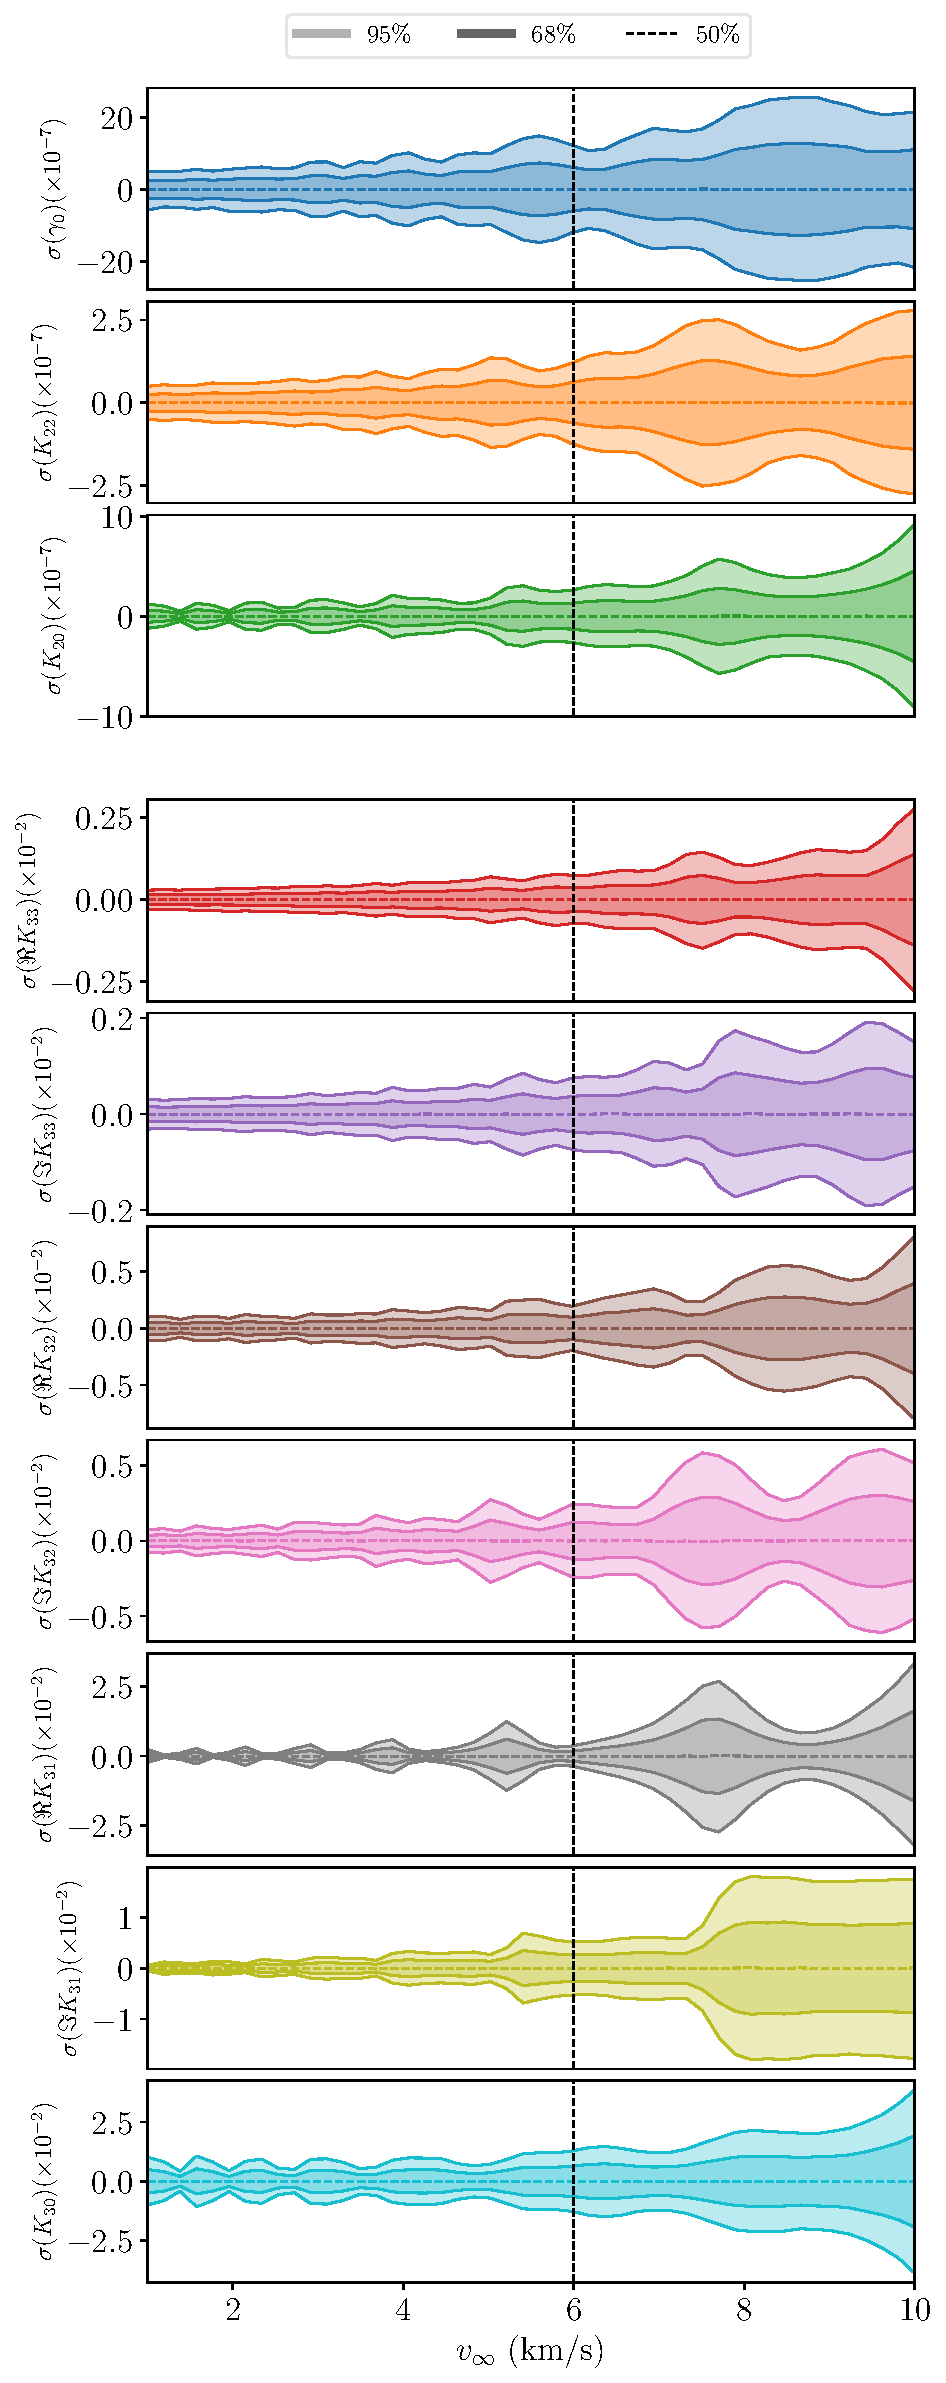
\includegraphics[height=0.89\textheight]{figs/scan-vex.pdf}
  \caption{1 and 2$\sigma$ confidence intervals for the first-order parameter PPDs (\textit{top}) and second-order parameters (\textit{bottom}) as a function of orbital excess velocity $v_\infty$. The vertical dashed line indicates the reference asteroid value of 6 km s$^{-1}$. The red vertical lines indicate when $\sigma = 0.01$.}
  \label{fig:scan-vex}
\end{figure}

Figure \ref{fig:scan-vex} demonstrates that parameter precision does not depend strongly on excess velocity, aside from a slight trend especially in the higher order parameters for uncertainty to increase with $v_\infty$. This is likely due to the fact that larger $v_\infty$ leads to a faster and flatter orbit with less time spent close to the planet, where tidal torque is strongest. There are also smaller-scale oscillations in the uncertainty, due to the orientation of the asteroid at perigee varying. The asteroid is always simulated to start at the same orientation, but increasing $v_\infty$ decreases the time to perigee, so that the asteroid enters this region of high torque at different orientations depending on $v_\infty$. This effect explains why these small-scale oscillations have the same period for all parameters. Note that these oscillations are sometimes large enough to raise $\sigma > 0.01$, shown by the red vertical line.

\begin{figure}
  \centering
  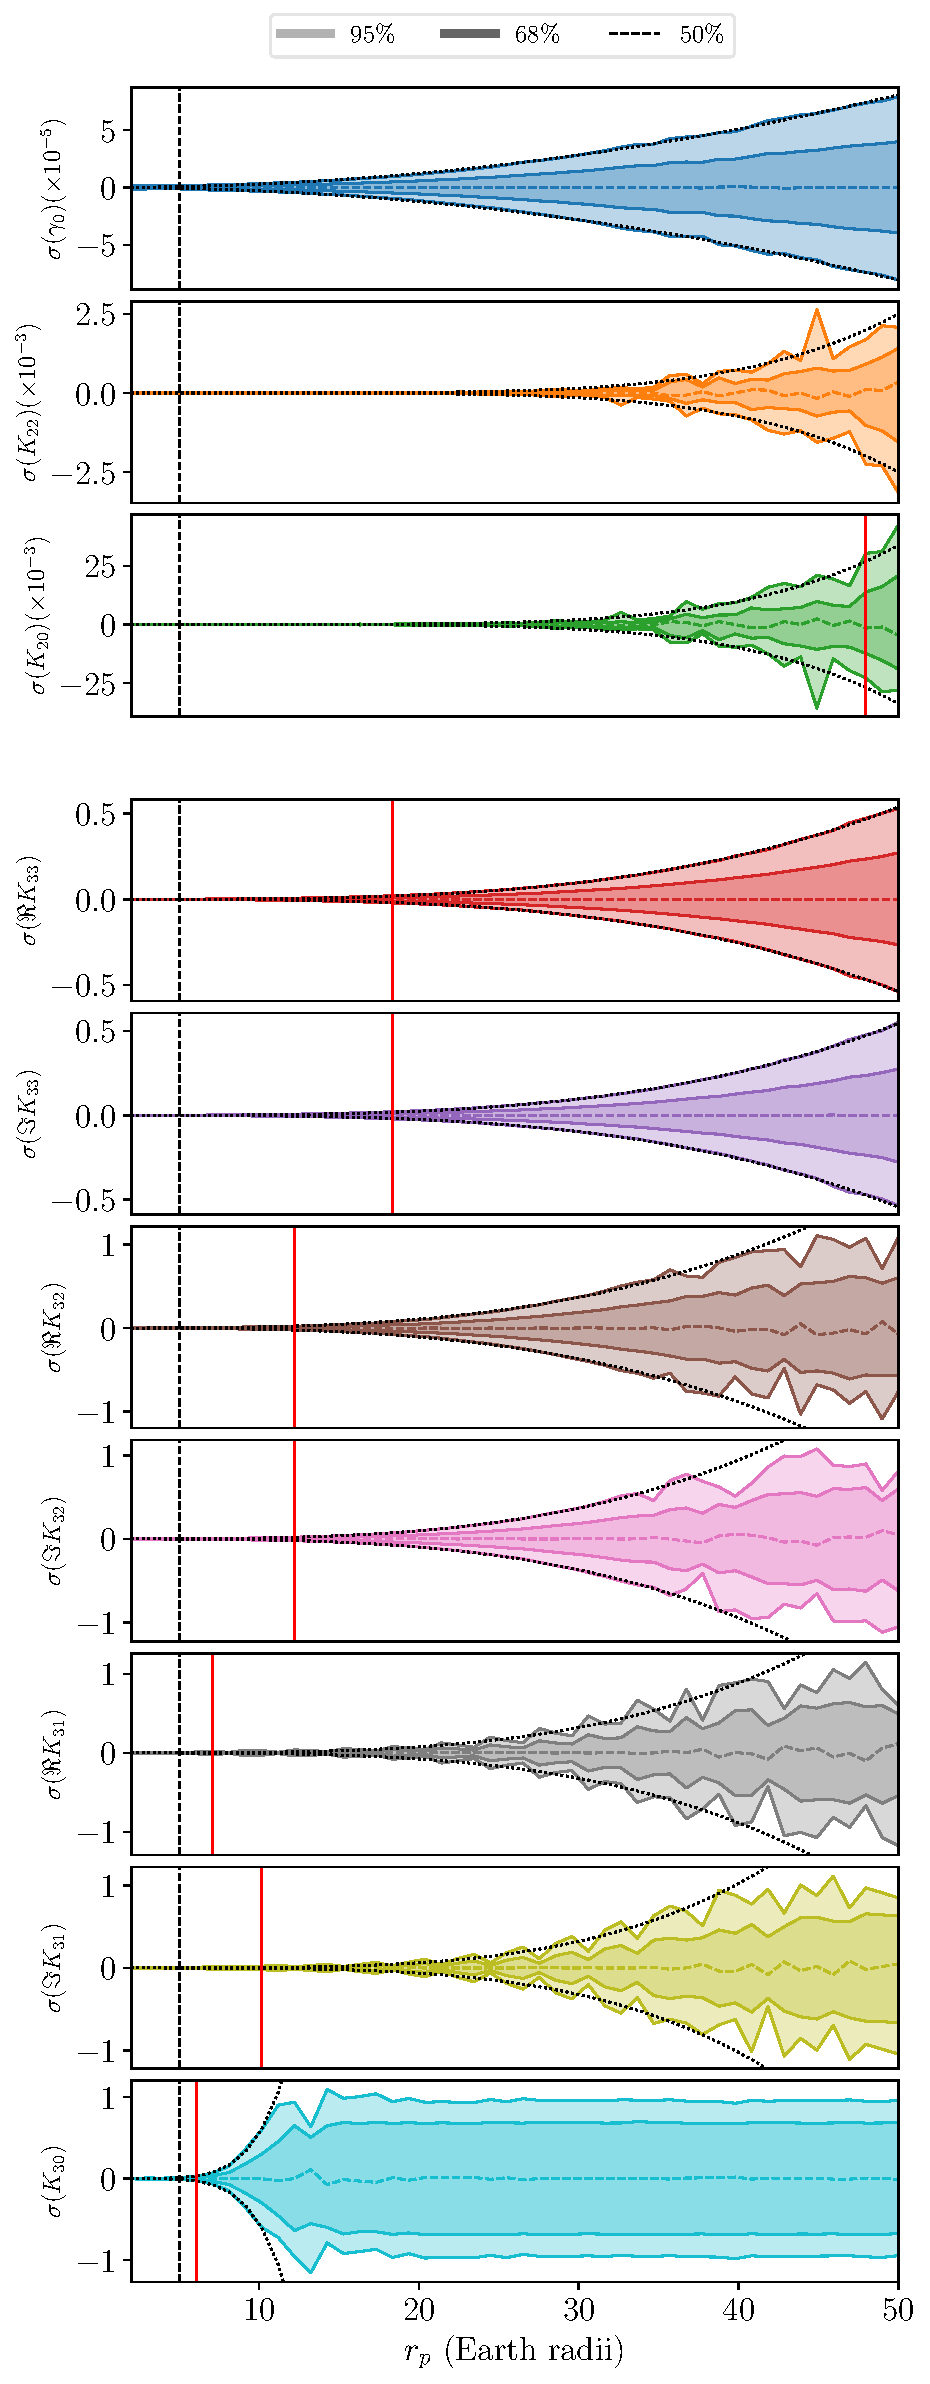
\includegraphics[height=0.89\textheight]{figs/scan-perigee.pdf}
  \caption{1 and 2$\sigma$ confidence intervals for the first-order parameter PPDs (\textit{top}) and second-order parameters (\textit{bottom}) as a function of perigee distance $r_p$. The vertical dashed line indicates the reference asteroid value of 5 Earth radii. The dotted curve indicates a power-law fit (see text). The red vertical lines indicate when $\sigma = 0.01$.}
  \label{fig:scan-perigee}
\end{figure}

Figure \ref{fig:scan-perigee} shows much stronger dependence of parameter uncertainty on perigee distance, as expected by the factor of $(a_\mathcal{A}/D)^{\ell'}$ present in equation \ref{eqn:tidal-torque} and mentioned in section \ref{sec:tidal-torque}. For $r_p \approx 6$ or 7 Earth radii, $\sigma(K_{30})$ reaches the reference 0.01 limit. At slightly higher $r_p$, $K_{31}$ and $K_{32}$ become similarly unresolved, and at $r_p \approx 20$ Earth radii, $K_{33}$, the last second-order component, becomes unresolved. Even before this, at $r_p \approx 10$ Earth radii, the most uncertain parameter $K_{30}$ fills the prior distribution with uncertainty ranging from -1 to 1, visible by the sudden cut-off in uncertainty increase and the discontinuity of the $\sigma$ curve there. The location of these limits will change if different encounter properties are used, but this is still an illustrative example.

\begin{table}
  \centering
  \begin{tabular}{l|c}
    \hline
    Parameter & $\alpha$ \\ \hline
    $\gamma_0$ & $2.05$ \\
    $K_{22}$ & $5.47$ \\
    $K_{20}$ & $5.47$ \\ \hline
    $\Re K_{33}$ & $3.35$ \\
    $\Im K_{33}$ & $3.37$ \\
    $\Re K_{32}$ & $3.05$ \\
    $\Im K_{32}$ & $3.27$ \\
    $\Re K_{31}$ & $3.53$ \\
    $\Im K_{31}$ & $4.02$ \\
    $K_{30}$ & $5.75$ \\ \hline
  \end{tabular}
  \caption{Power law slope values for the dependence of parameter uncertainty on perigee distance $r_p$. Slope is defined by $\sigma \propto r_p^\alpha$.}
  \label{tab:scan-perigee-alpha}
\end{table}

Fitted to each of the curves in figure \ref{fig:scan-perigee} are power law uncertainties $\sigma \propto r_p^\alpha$. These fits were performed via the method of least squares, and all data with $\sigma > 0.7$ was removed due to its sensitivity to the arbitrarily-chosen boundary of the prior. The values of $\alpha$ are shown in table \ref{tab:scan-perigee-alpha}. These slope values express how much each parameter is dependent on $r_p$. It is observed that $\gamma_0$ is least dependent on $r_p$, with $\sigma(\gamma_0) \sim r_p^2$. The other two first-order parameters are much more strongly dependent, with $\sigma \sim r_p^{5.5}$. The second-order parameters have milder slopes between 3 and 4 (except for $K_{30}$) which is fortunate from the perspective of making precise observations, since lower $\alpha$ renders larger values of $r_p$ accessible to measuring $K_{3m}$.

The axes of figure \ref{fig:scan-perigee} show that parameters with large $m$ are more precisely determined than parameters with small $m$, as can be seen by comparing $K_{22}$ to $K_{20}$ and comparing $K_{33}$ to other $K_{3m}$ values. Large $m$ moments correspond to moments that control higher frequency fluctuations in density at the asteroid equator. This pattern of large $m$ corresponding to low uncertainty is a general trend and will be seen in the following sections as well.

The very strong dependence of $\sigma$ on $r_p$ makes this analysis only to extract second-order moments on close encounters. Fortunately, in the case of Earth, these encounters are also likely to have the best associated observational uncertainty when above the horizon due to their proximity. The first-order moments can still be extracted at much larger perigee distances in our model.


\subsection{Observational Uncertainty}
\label{sec:scan-uncertainty}
There are two parameters, $\sigma_\theta$ and $\sigma_\rho$, which govern the observational uncertainty of the data set (defined in section \ref{sec:uncertainty}). Rather than explore the full space spanned by these two values, we measure how parameter uncertainties depend on the product of uncertainties $\sigma_\theta\sigma_\rho$ (with the radio fixed), and the ratio $\sigma_\rho / \sigma_\theta$ (with the product fixed).

We choose these metrics because we generally expect that the parameter uncertainty $\sigma$ be proportional to the observational uncertainty, but whether the dependence is stronger on $\sigma_\theta$ or $\sigma_\rho$ is not immediately clear. We get around this problem by varying $\sigma_\theta$ and $\sigma_\rho$ together and fixing their ratio, and measuring the posterior uncertainty $\sigma$, with $\sigma/\sigma_\theta$ shown in figure \ref{fig:scan-product}. Indeed, we find that $\sigma \propto \sigma_\theta$ almost exactly, and since $\sigma_\rho / \sigma_\theta$ is fixed, we also have $\sigma \propto \sigma_\rho$. For large $\sigma_\theta \sigma_\rho$, the proportionality fails, but this is because $\sigma(K_{30}) \approx 1$ which fills the prior. Uncertainty cannot increase beyond this value.

\begin{figure}
  \centering
  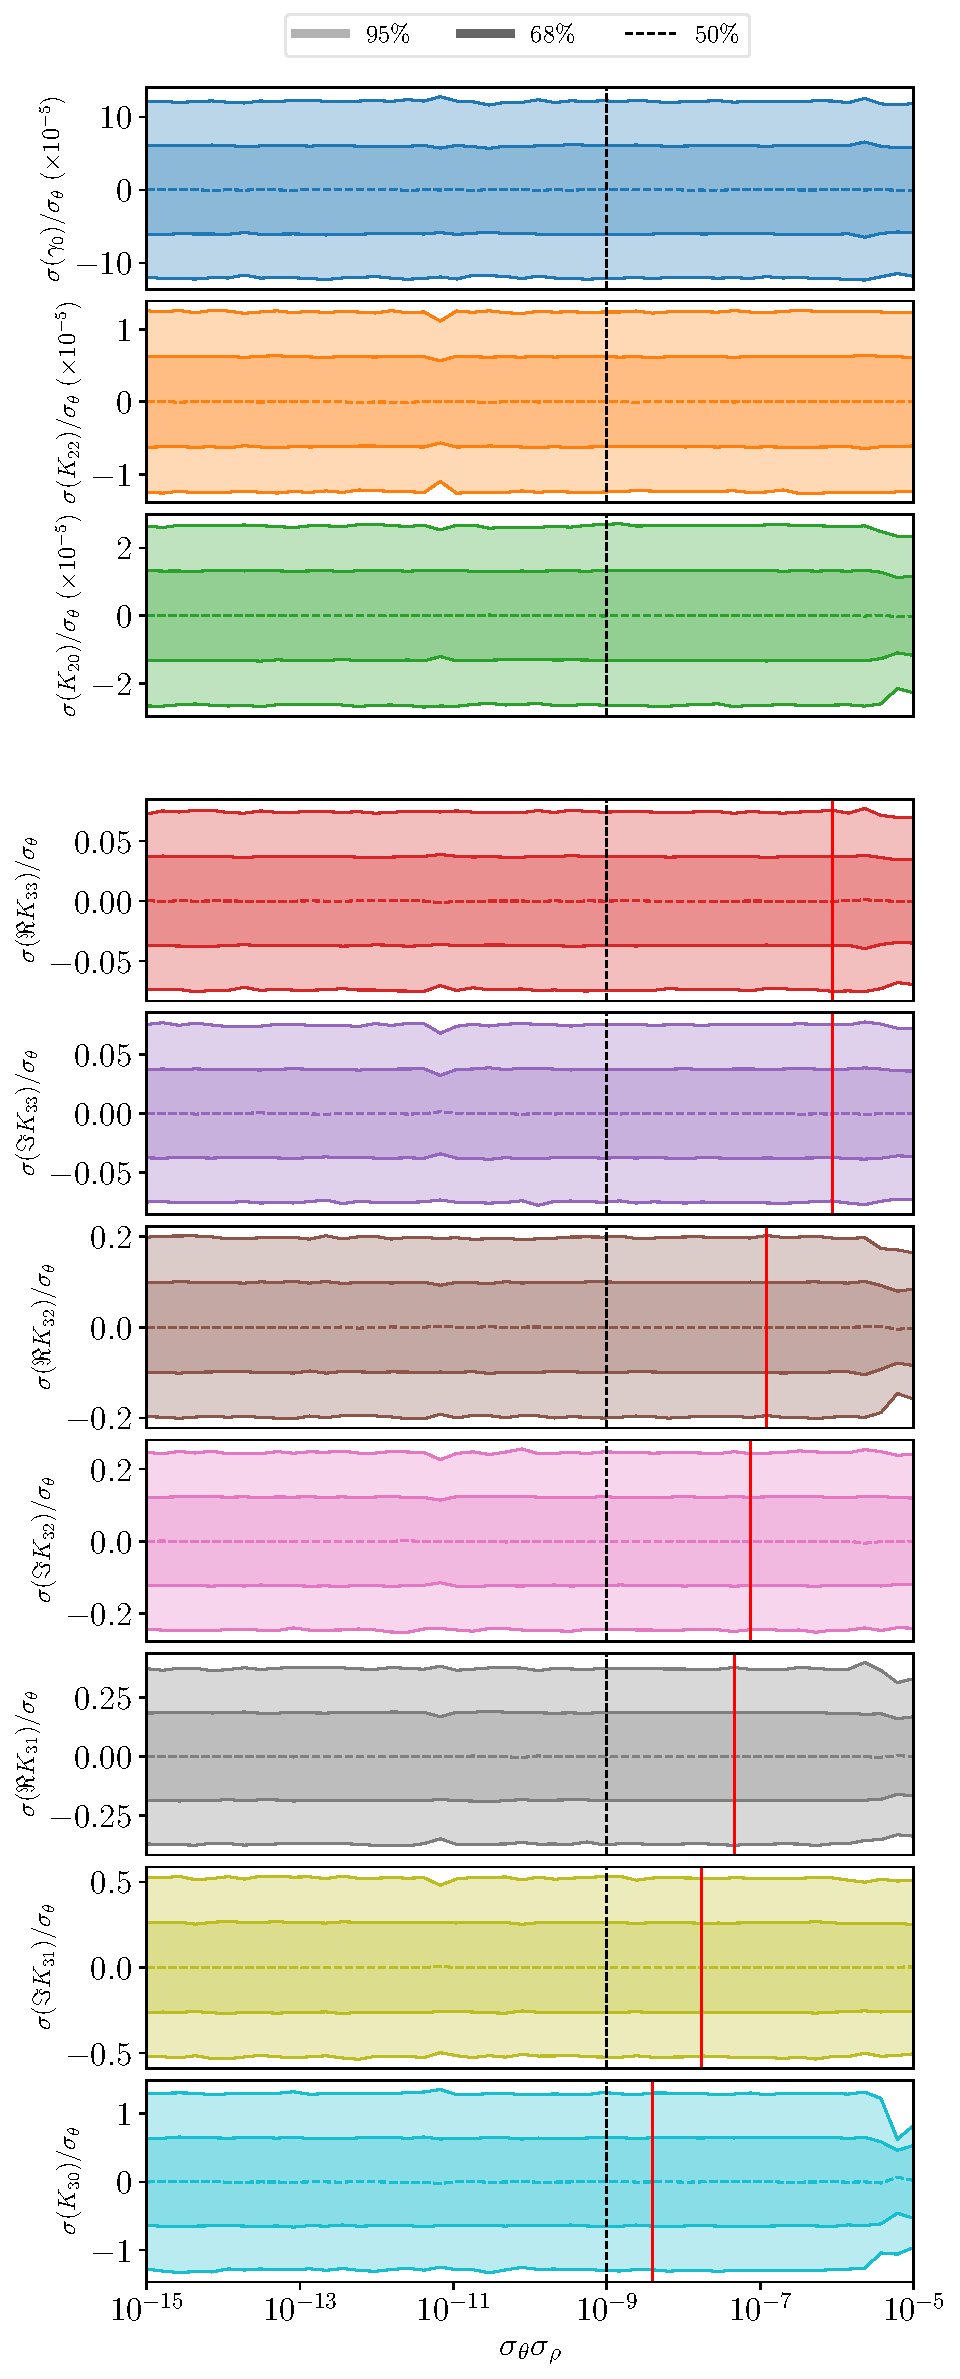
\includegraphics[height=0.89\textheight]{figs/scan-product.pdf}
  \caption{1 and 2$\sigma$ confidence intervals divided by $\sigma_\theta$ for the first-order parameter PPDs (\textit{top}) and second-order parameters (\textit{bottom}) as a function of observational uncertainty product $\sigma_\theta \sigma_\rho$. The vertical dashed line indicates the reference asteroid value of $10^{-9}$. The red vertical lines indicate when $\sigma =0.01$.}
  \label{fig:scan-product}
\end{figure}

We also investigate the dependence of posterior uncertainty on $\sigma_\rho / \sigma_\theta$ with $\sigma_\theta \sigma_\rho$ fixed in figure \ref{fig:scan-ratio}. If we simply had $\sigma \propto \sigma_\theta \sigma_\rho$, then $\sigma$ would have no dependence on $\sigma_\rho / \sigma_\theta$. Any deviation from constant $\sigma$ shown in the figure therefore reveals some additional dependence in the model on one of the observational uncertainties.

\begin{figure}
  \centering
  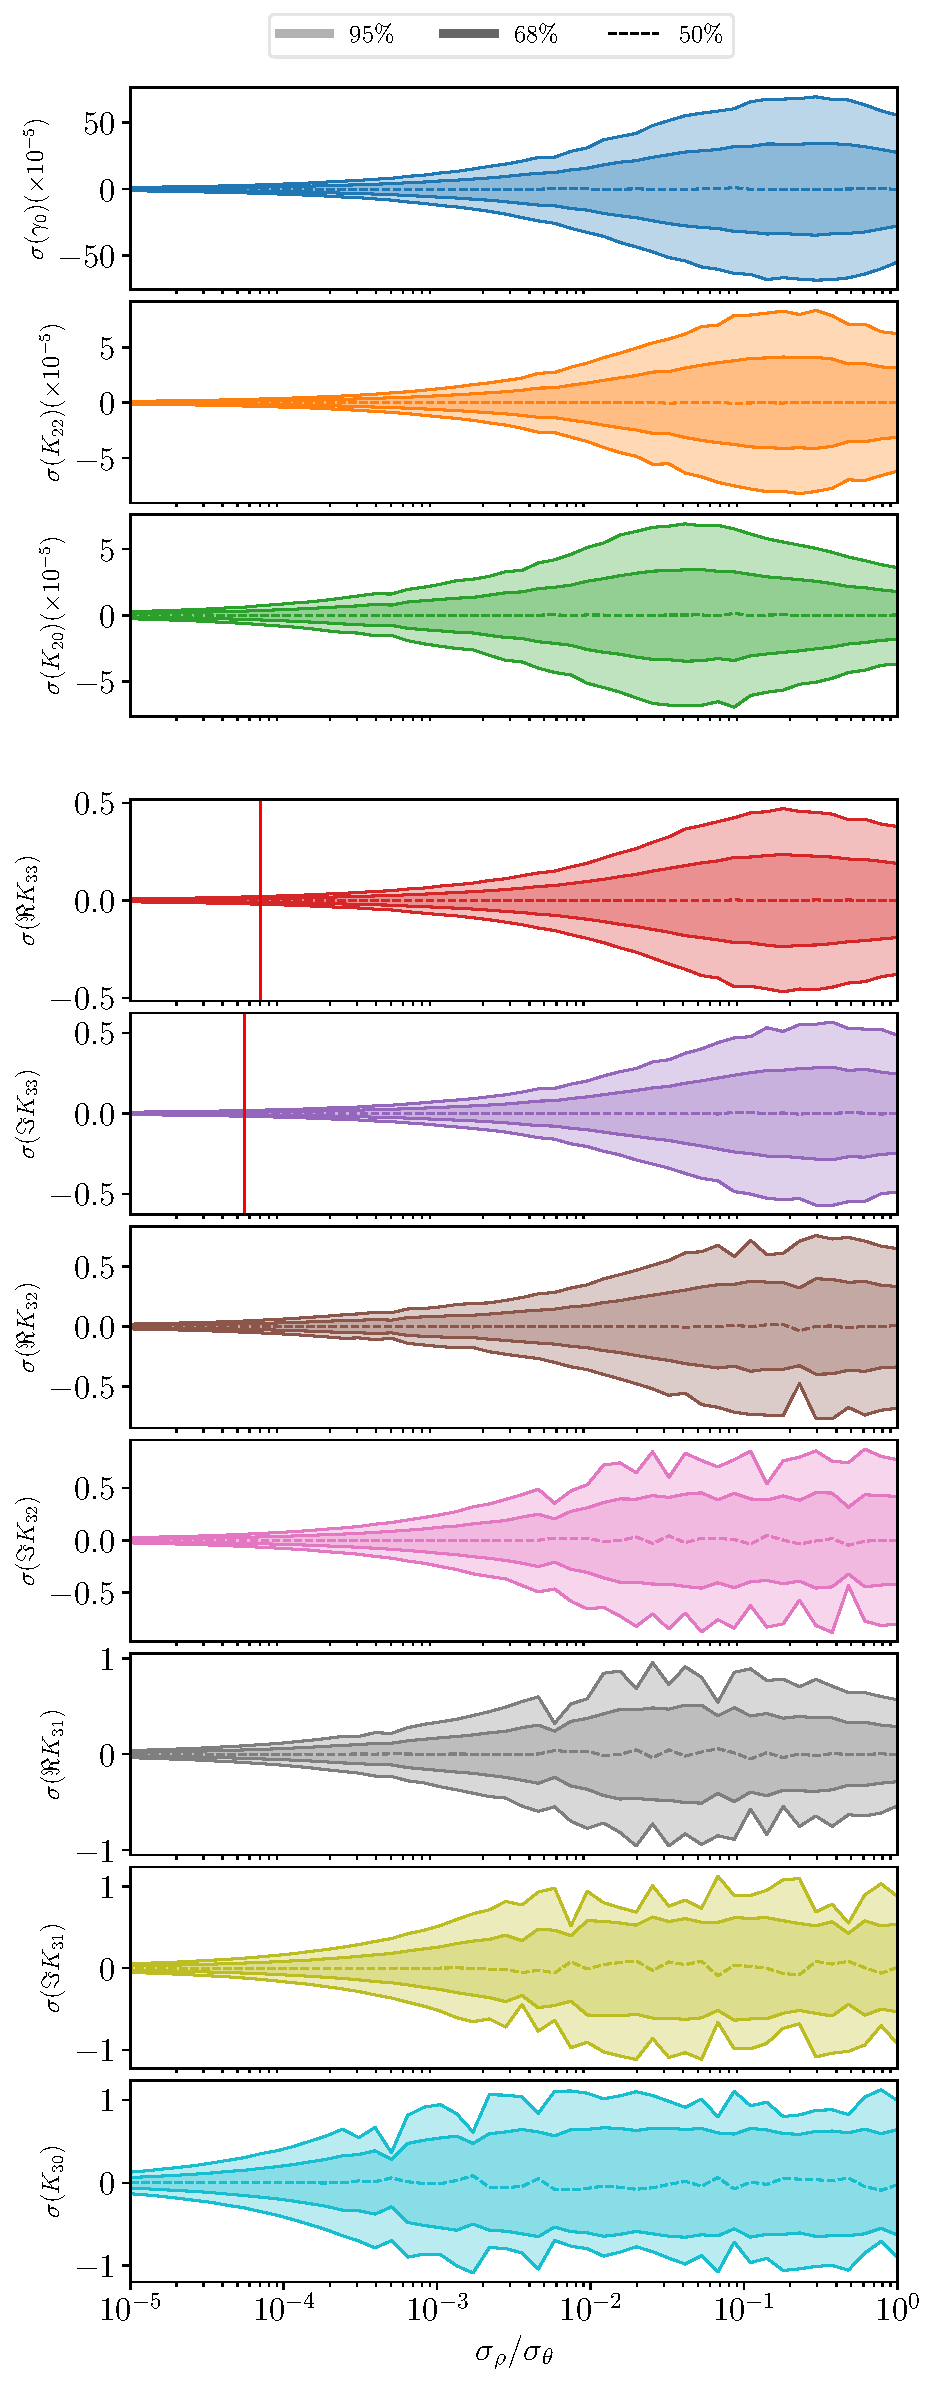
\includegraphics[height=0.89\textheight]{figs/scan-ratio.pdf}
  \caption{1 and 2$\sigma$ confidence intervals for the first-order parameter PPDs (\textit{top}) and second-order parameters (\textit{bottom}) as a function of observational uncertainty ratios $\sigma_\rho / \sigma_\theta$. The reference asteroid value is $\sigma_\rho/ \sigma_\theta =10^{-5}$. The red vertical lines indicate when $\sigma = 0.01$. (Lines are not shown for $K_{3m}$, $m < 3$ because they coincide with the vertical axis.)}
  \label{fig:scan-ratio}
\end{figure}

Indeed, figure  \ref{fig:scan-ratio} shows increased uncertainty when $\sigma_\rho/\sigma_\theta$ is large, so that $\sigma$ depends more on $\sigma_\rho$ than on $\sigma_\theta$. We summarize this pattern by stating that, if the observer had to choose between better precision on the period or on the spin pole of the data, they should choose period. This is fortunate for observers since, \jtd{I want to say that precision on the period is better constrained by light curve analysis, but I do not know enough about light curve analysis to be sure.}

Another conclusion that can be drawn from figure \ref{fig:scan-ratio} is that $\sigma(\sigma_\rho/\sigma_\theta)$ is proportional for all $K_{\ell m}$. The proportionality constant shows the same dependence on $\ell$ and $m$ mentioned previously. The proportionality is broken near $\sigma \approx \pm 1$, where $\sigma$ fills the prior.

The location of the $\sigma > 0.01$ limit demonstrates the great influence of observational precision on fit uncertainty; increasing $\sigma_\theta \sigma_\rho$ or $\sigma_\rho / \sigma_\theta$ by even a small amount raises $\sigma(K_{3m}) > 0.01$ in most cases.



\subsection{Asteroid shape}
\label{sec:scan-shape}

The true values of $K_{\ell m}$, $\gamma_0$, and $a_\mathcal{A}$ affect the uncertainties in extracted density moments $\sigma$. Here, we only investigate the sensitivity of $\sigma$ to the first-order parameters and $a_\mathcal{A}$. The $K_{2m}$ moments can therefore also be viewed as the axes of a uniform density triaxial ellipsoid (equation \ref{eqn:ellipsoid-axes}).

In figure \ref{fig:scan-space-sigma}, we show the 1$\sigma$ confidence intervals as a function of $K_{20}$ and $K_{22}$, or alternatively $a/c$ and $b/c$. We use axis ratios rather than the values of $a$, $b$, and $c$ to remove the $a_\mathcal{A}$ dependence of equation \ref{eqn:ellipsoid-axes}. The figure shows large uncertainty in $\gamma_0$ for $K_{22}=0$, or $a/c=b/c$, because $K_{20}$ is rotationally symmetric around $\unit z$, and $\gamma_0$ is the initial orientation with respect to the $\unit z$ axis. The data then have no physical dependence on $\gamma_0$ when $K_{22}=0$. This induces degeneracy in the model which inflates uncertainties, not only in $\gamma_0$ but also the other components.

\begin{figure*}
  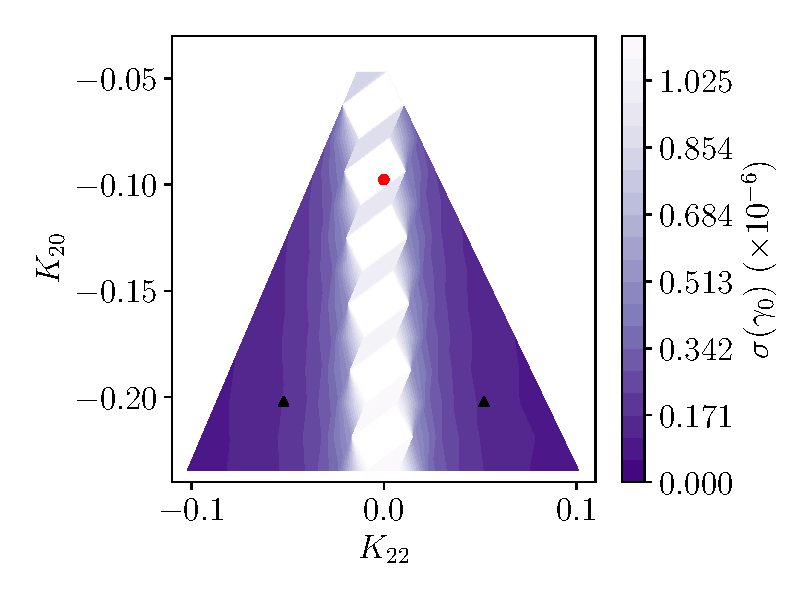
\includegraphics[width=0.33\textwidth]{figs/probe-space-theta-1-sigma.pdf}\hfill
  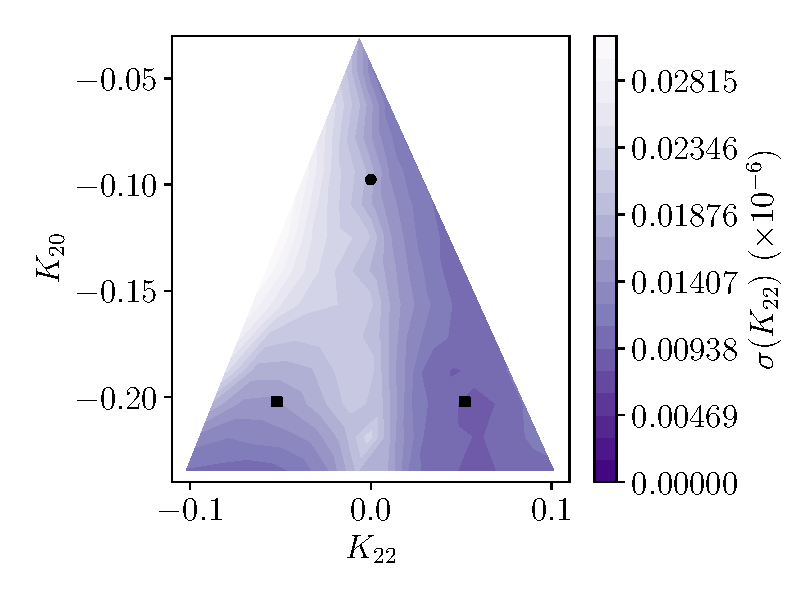
\includegraphics[width=0.33\textwidth]{figs/probe-space-theta-2-sigma.pdf}\hfill
  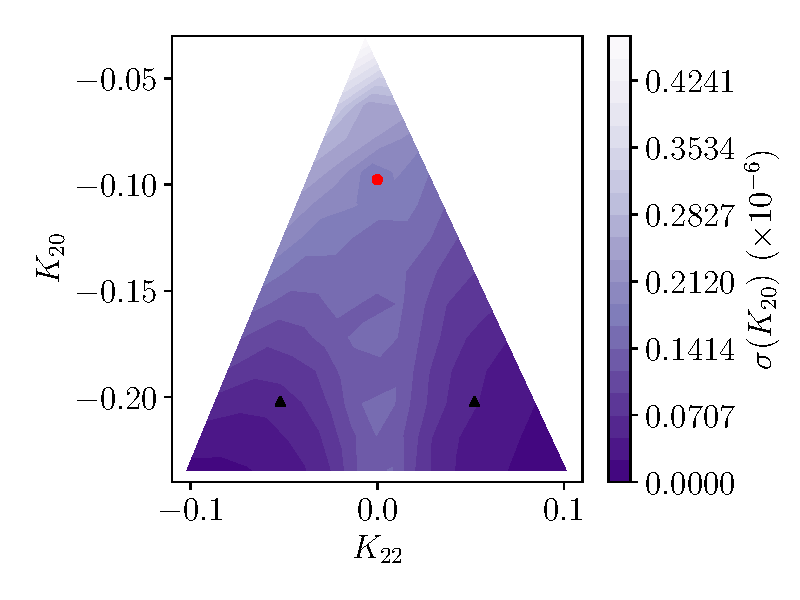
\includegraphics[width=0.33\textwidth]{figs/probe-space-theta-3-sigma.pdf}

  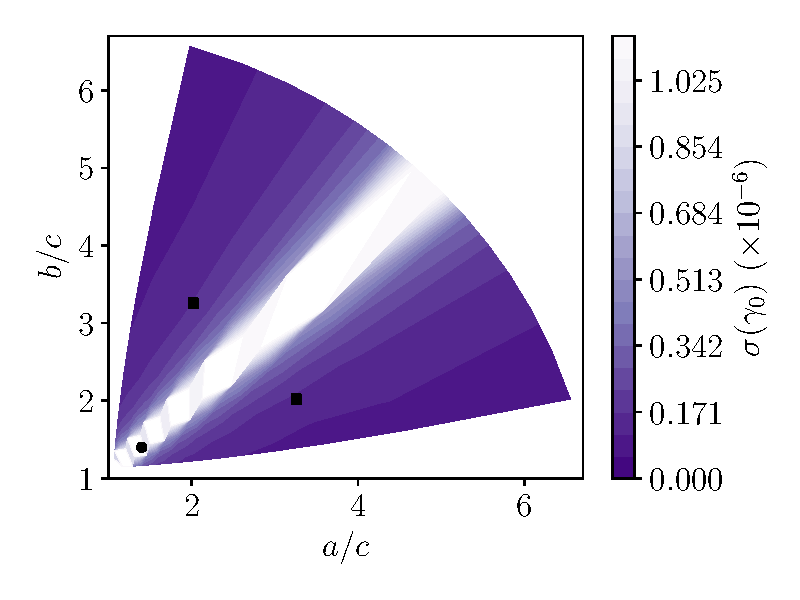
\includegraphics[width=0.33\textwidth]{figs/probe-space-ab-1-sigma.pdf}\hfill
  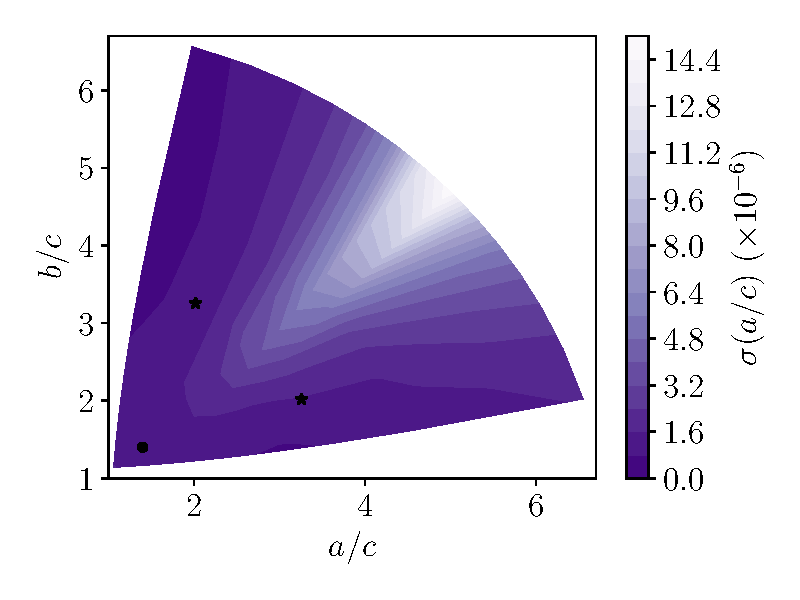
\includegraphics[width=0.33\textwidth]{figs/probe-space-ab-a-sigma.pdf}\hfill
  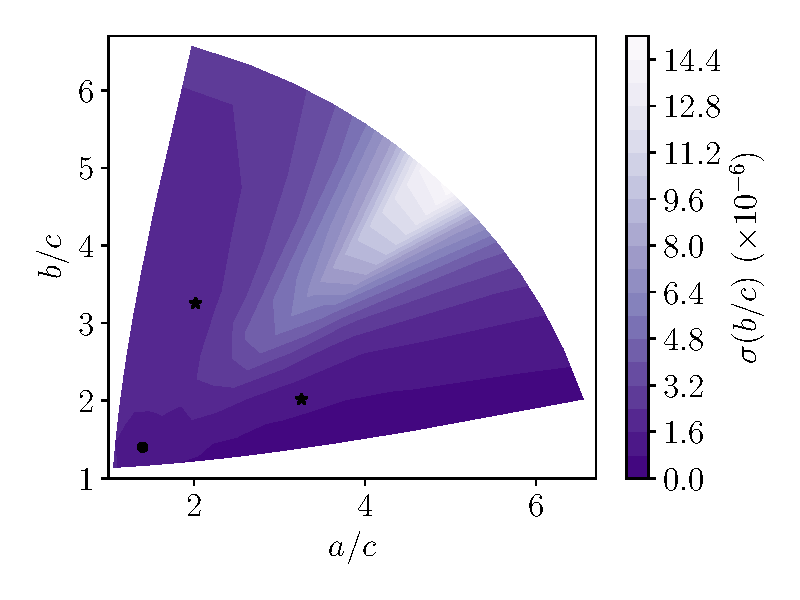
\includegraphics[width=0.33\textwidth]{figs/probe-space-ab-b-sigma.pdf}

  \caption{1$\sigma$ confidence interval for fit parameters $\gamma_0$, $K_{22}$, and $K_{20}$ (\textit{top row}) and $\gamma_0$, $a/c$, and $b/c$ (\textit{bottom row}). Also shown as black points are the reference asteroid shapes; the symmetric case is marked with a red circle and the asymmetric with a black triangle.}
  \label{fig:scan-space-sigma}
\end{figure*}

To remove the inflated uncertainty, one could assume a rotationally symmetric asteroid, remove $\gamma_0$ as a parameter, and run a fit. For a nearly rotationally symmetric asteroid however, a new parametrization is necessary which does not contain the ill-constrained $\gamma_0$ parameter. This task is beyond the scope of this paper, so we mostly consider asymmetric asteroids throughout.

Figure \ref{fig:scan-space-sigma} also shows low uncertainty for highly asymmetric asteroids, where $b/c$ and $a/c$ are very different (i.e., when $|K_{22}|$ is large). Additionally, $\sigma(K_{20})$ and $\sigma(K_{22})$ decrease for large $|K_{20}|$, which corresponds to large axis ratios in the ellipsoid case.

Figure \ref{fig:scan-space-corr} displays the correlation between the first-order parameters for reference. They show that $\gamma_0$ and $K_{22}$ are often correlated for asymmetric asteroids, while $\gamma_0$ and $K_{20}$ are usually not. This is expected as $K_{22}$ is dependent on the orientation of the asteroid and $K_{20}$ is not. They also show that $K_{22}$ and $K_{20}$ are usually correlated, and that $a/c$ and $b/c$ are highly correlated. The latter is expected due to the $1/c$ dependence. As for the former, this correlation could likely be removed by an alternate parametrization, reducing uncertainties in the shape parameters.

\begin{figure*}
  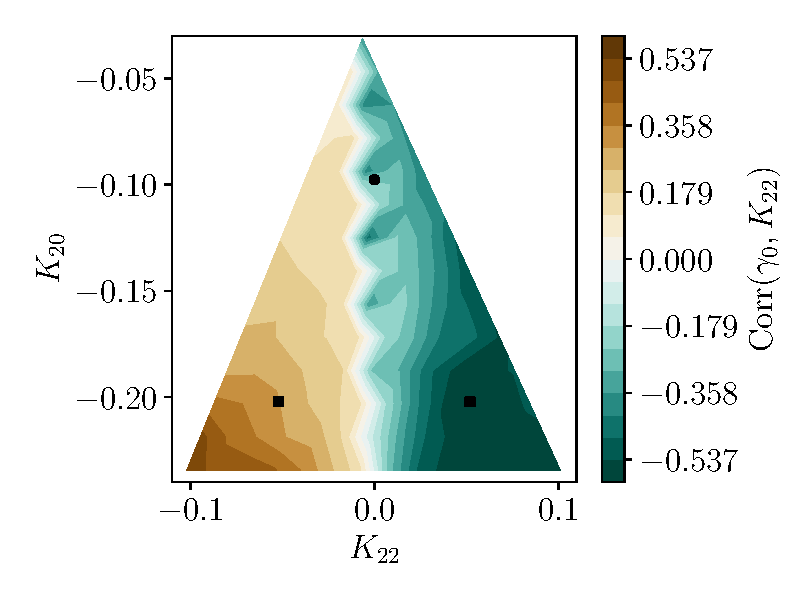
\includegraphics[width=0.33\textwidth]{figs/probe-space-corr12.pdf}\hfill
  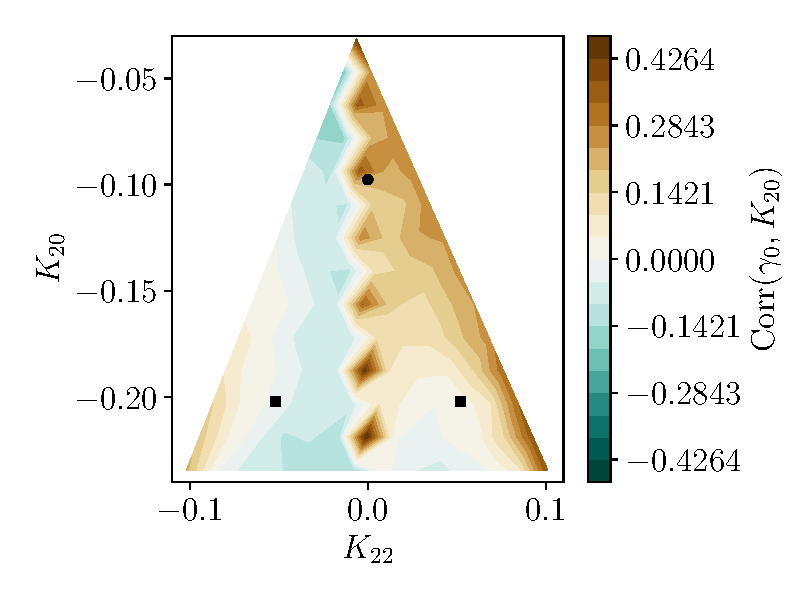
\includegraphics[width=0.33\textwidth]{figs/probe-space-corr13.pdf}\hfill
  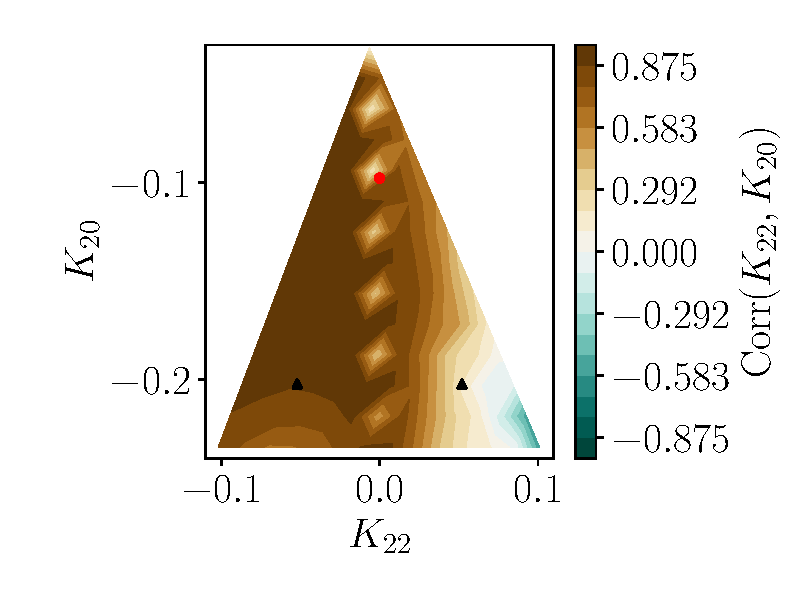
\includegraphics[width=0.33\textwidth]{figs/probe-space-corr23.pdf}

  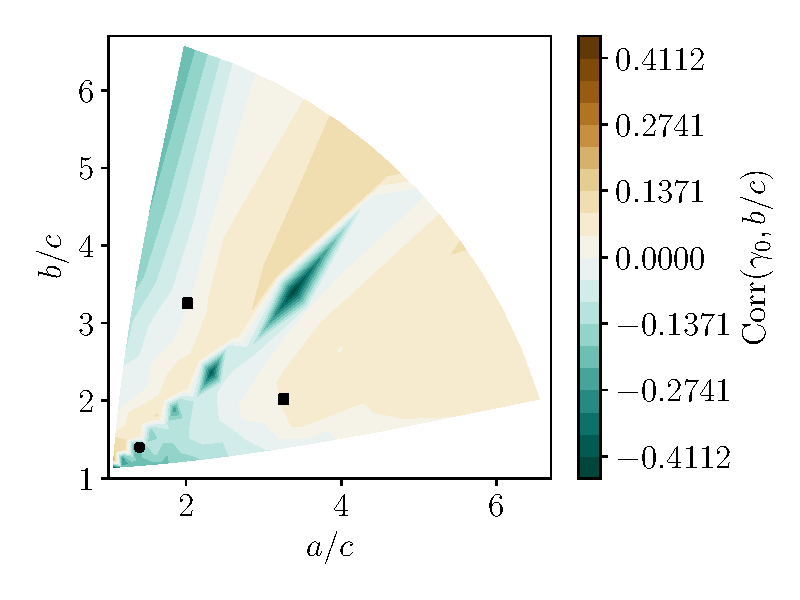
\includegraphics[width=0.33\textwidth]{figs/probe-space-ab-1b.pdf}\hfill
  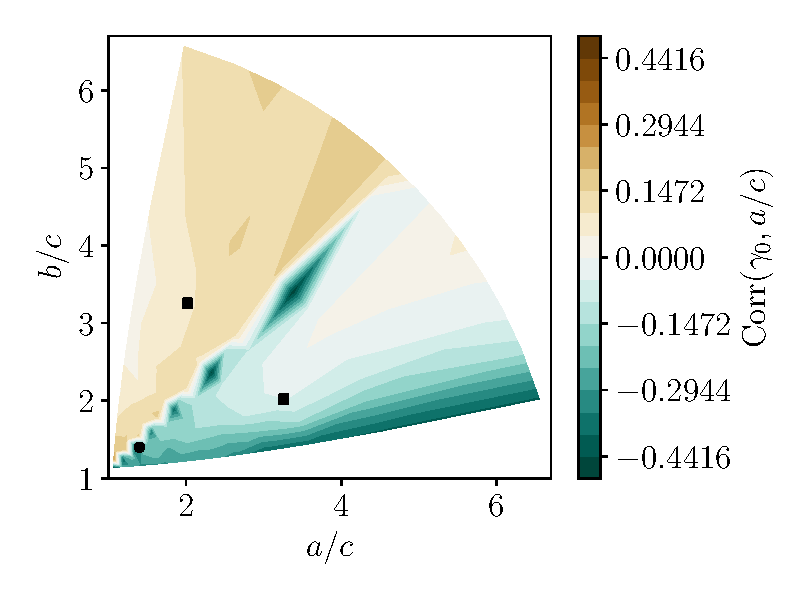
\includegraphics[width=0.33\textwidth]{figs/probe-space-ab-1a.pdf}\hfill
  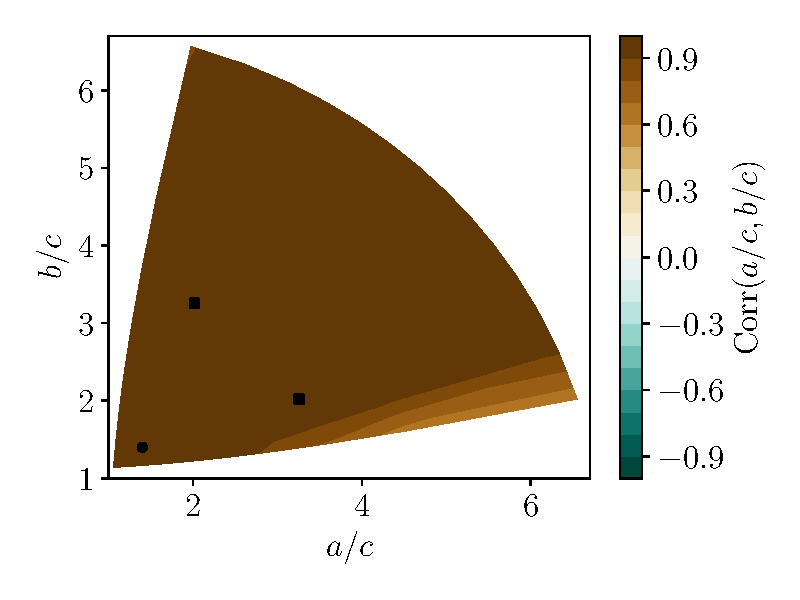
\includegraphics[width=0.33\textwidth]{figs/probe-space-ab-ab.pdf}
  
  \caption{Correlations between PPDs for fit parameters $\gamma_0$, $K_{22}$, and $K_{20}$ (\textit{top row}) and $\gamma_0$, $a/c$, and $b/c$ (\textit{bottom row}).  Also shown as black points are the reference asteroid shapes; the symmetric case is marked with a red circle and the asymmetric with a black triangle.}
  \label{fig:scan-space-corr}
\end{figure*}

Overall, the variation in the uncertainties on $K_{20}$ and $K_{22}$ (the first-order density moments) is present but largely smooth across their allowed parameter space, as is their correlation (except the large $K_{22}$ corner). It therefore seems reasonable to use the asymmetric asteroid shape as a stand-in for an unknown's asteroid shape when simulating an encounter, as we do in this paper. The uncertainty then can be expected to differ across other shapes by a factor of about two or less, as long as the degenerate, symmetric asteroid regime is avoided.

On the other hand, the posterior uncertainty of $K_{3m}$ is much more strongly dependent on asteroid length $a_\mathcal{A}$. Figure \ref{fig:scan-am} displays posterior uncertainty $\sigma$ as a function of $a_\mathcal{A}$, defined in equation \ref{eqn:am}. The vertical axis is shown in log space, meaning that the average of the upper and lower error bars of $\sigma$ is shown instead of showing both as is done in other figures.

\begin{figure}
  \centering
  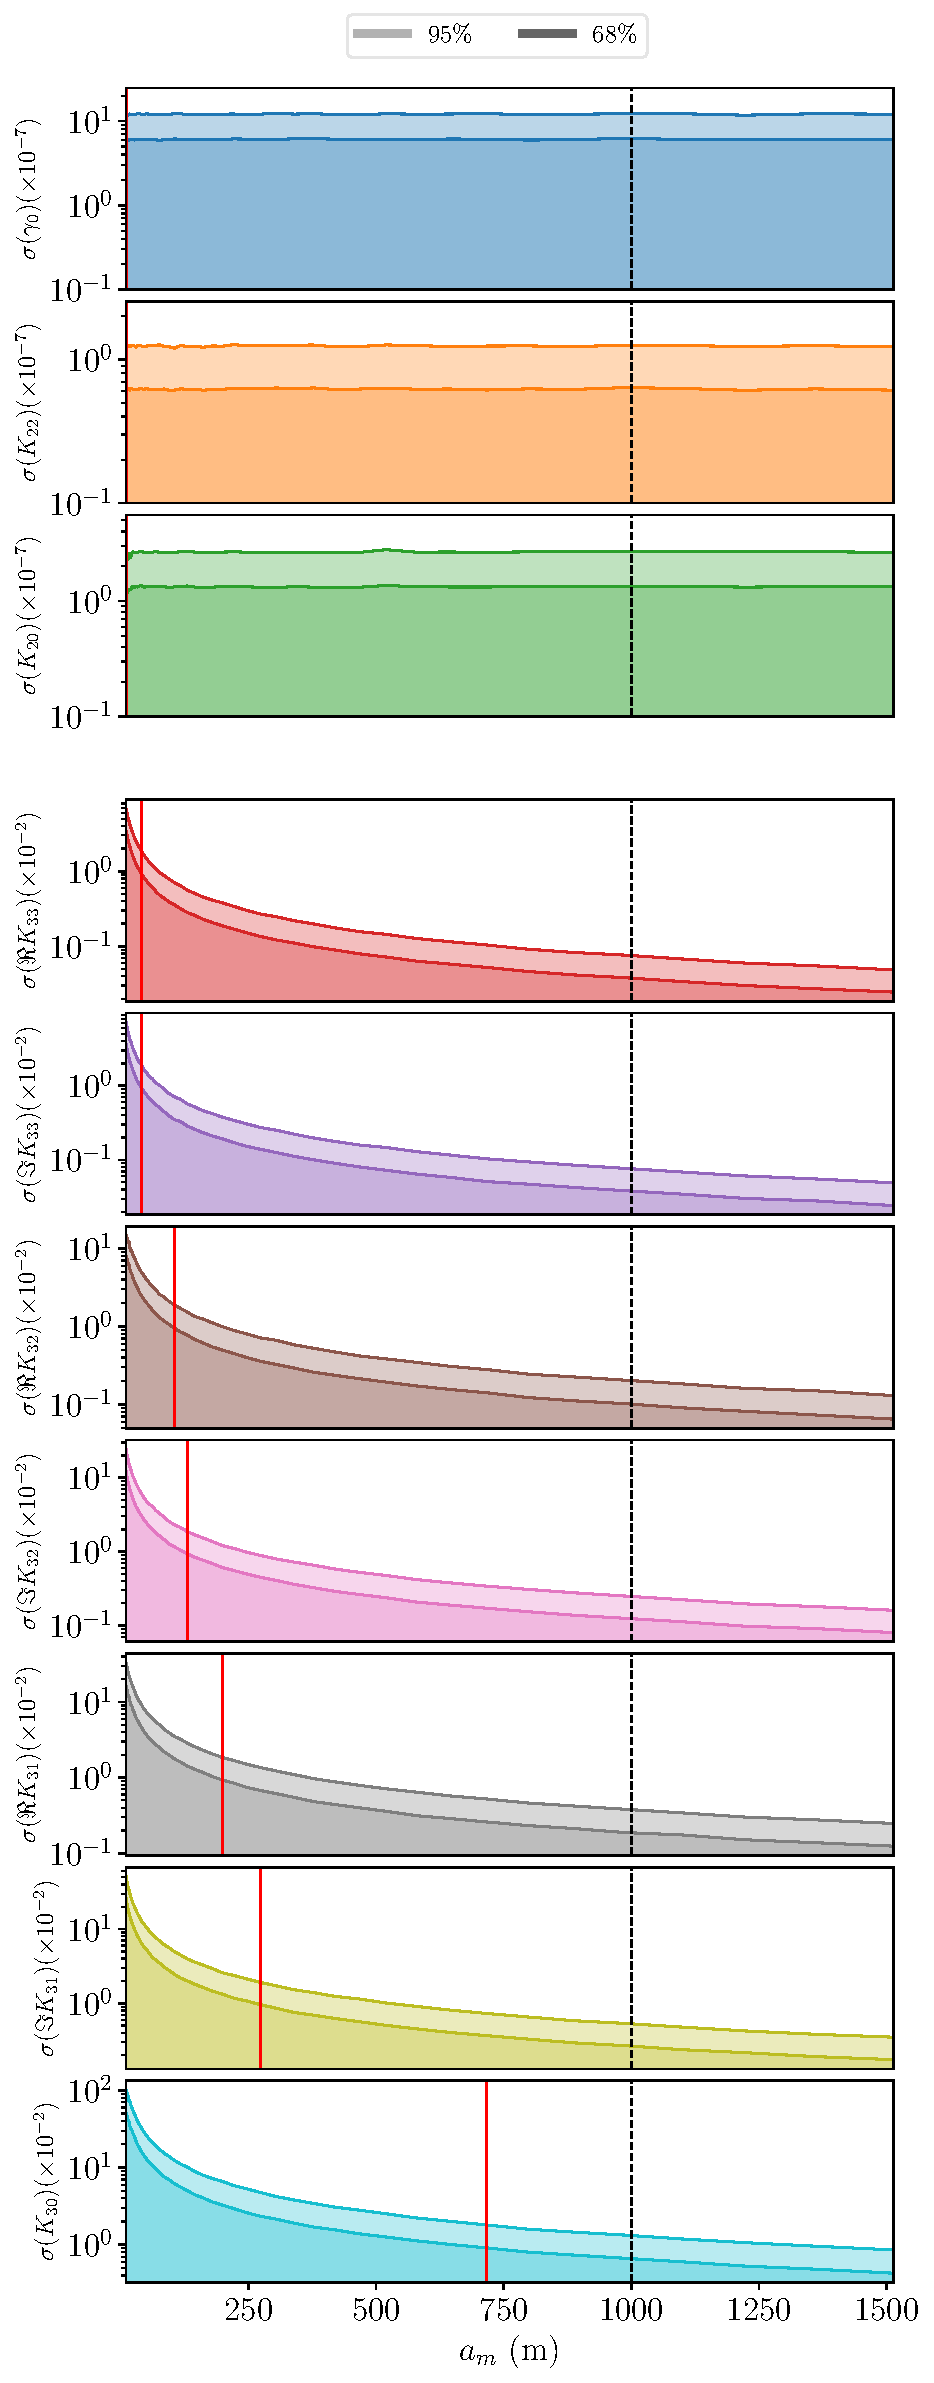
\includegraphics[height=0.89\textheight]{figs/scan-am.pdf}
  \caption{1 and 2$\sigma$ confidence intervals for the first-order parameter PPDs (\textit{top}) and second-order parameters (\textit{bottom}) as a function of asteroid length $a_\mathcal{A}$. The reference cadence is 2 minutes. The red vertical lines indicate when $\sigma = 0.01$. The black dashed line indicates the reference value of $a_\mathcal{A}=1000$ m.}
  \label{fig:scan-am}
\end{figure}

As was mentioned in section \ref{sec:tidal-torque}, the $K_{2m}$ parameters are insensitive to $a_\mathcal{A}$ since the $a_\mathcal{A}^2$ term in $\bm \tau$ (equation \ref{eqn:tidal-torque}) is canceled by the $a_\mathcal{A}^2$ in the moment of inertia (equation \ref{eqn:moi}). The $K_{3m}$ uncertainty is strongly dependent on $a_\mathcal{A}$ for the same reason that uncertainty is strongly dependent on $r_p$: the $(a_\mathcal{A}/D)^{\ell'}$ dependence of equation \ref{eqn:tidal-torque}. At $a_\mathcal{A} \lesssim 700$ m, $K_{30}$ becomes unresolved. The other parameters become unresolved for $a_\mathcal{A} \lesssim 300$ m, with the cut-off for $K_{33}$ being less than 100 meters. This $a_\mathcal{A}$ cut-off is quite sharp; figure \ref{fig:scan-am} shows steep decrease in $\sigma(a_\mathcal{A})$ for low $a_\mathcal{A}$, with an approximate functional form of $\sigma(a_\mathcal{A}) \sim e^{(a_\mathcal{A}/C)^p}$ for a scaling constant $C$ and some power $p < 1$. (In figure \ref{fig:scan-am}, the best fitting values are $p < 0.1$.) This sharpness indicates that the cut-off value of $a_\mathcal{A}$ is unlikely to change significantly if other parameters of the flyby are altered in a way that slightly increases or decreases $\sigma$. It therefore appears that extracting precise $K_{30}$ from asteroids with $a_\mathcal{A} \lesssim 700$ m is very unlikely with this analysis, and for $a_\mathcal{A} \lesssim 50$ m, all $K_{3m}$ will likely be unresolved.

For uniform density asteroids, large $a_\mathcal{A}$ is equivalent to large asteroid radius, which was mentioned in section \ref{sec:moments} and explicitly shown in equation \ref{eqn:ellipsoid-axes}. In non-uniform density asteroids, large $a_\mathcal{A}$ can also be achieved by distributing the mass of the asteroid near the surface, because the $r^2$ term in the integrand of the definition of $a_\mathcal{A}$ causes the density of regions distant from the asteroid centre of mass to dominate $a_\mathcal{A}$.




\subsection{Cadence}
\label{sec:scan-cadence}

The time between observations of asteroid angular velocity, or cadence, may vary depending on the observational schedule of the observing telescopes and the path of the asteroid through the sky.  We measure how the posterior uncertainty $\sigma$ varies with cadence ranging from two minutes to one hour in figure \ref{fig:scan-cadence}.

\begin{figure}
  \centering
  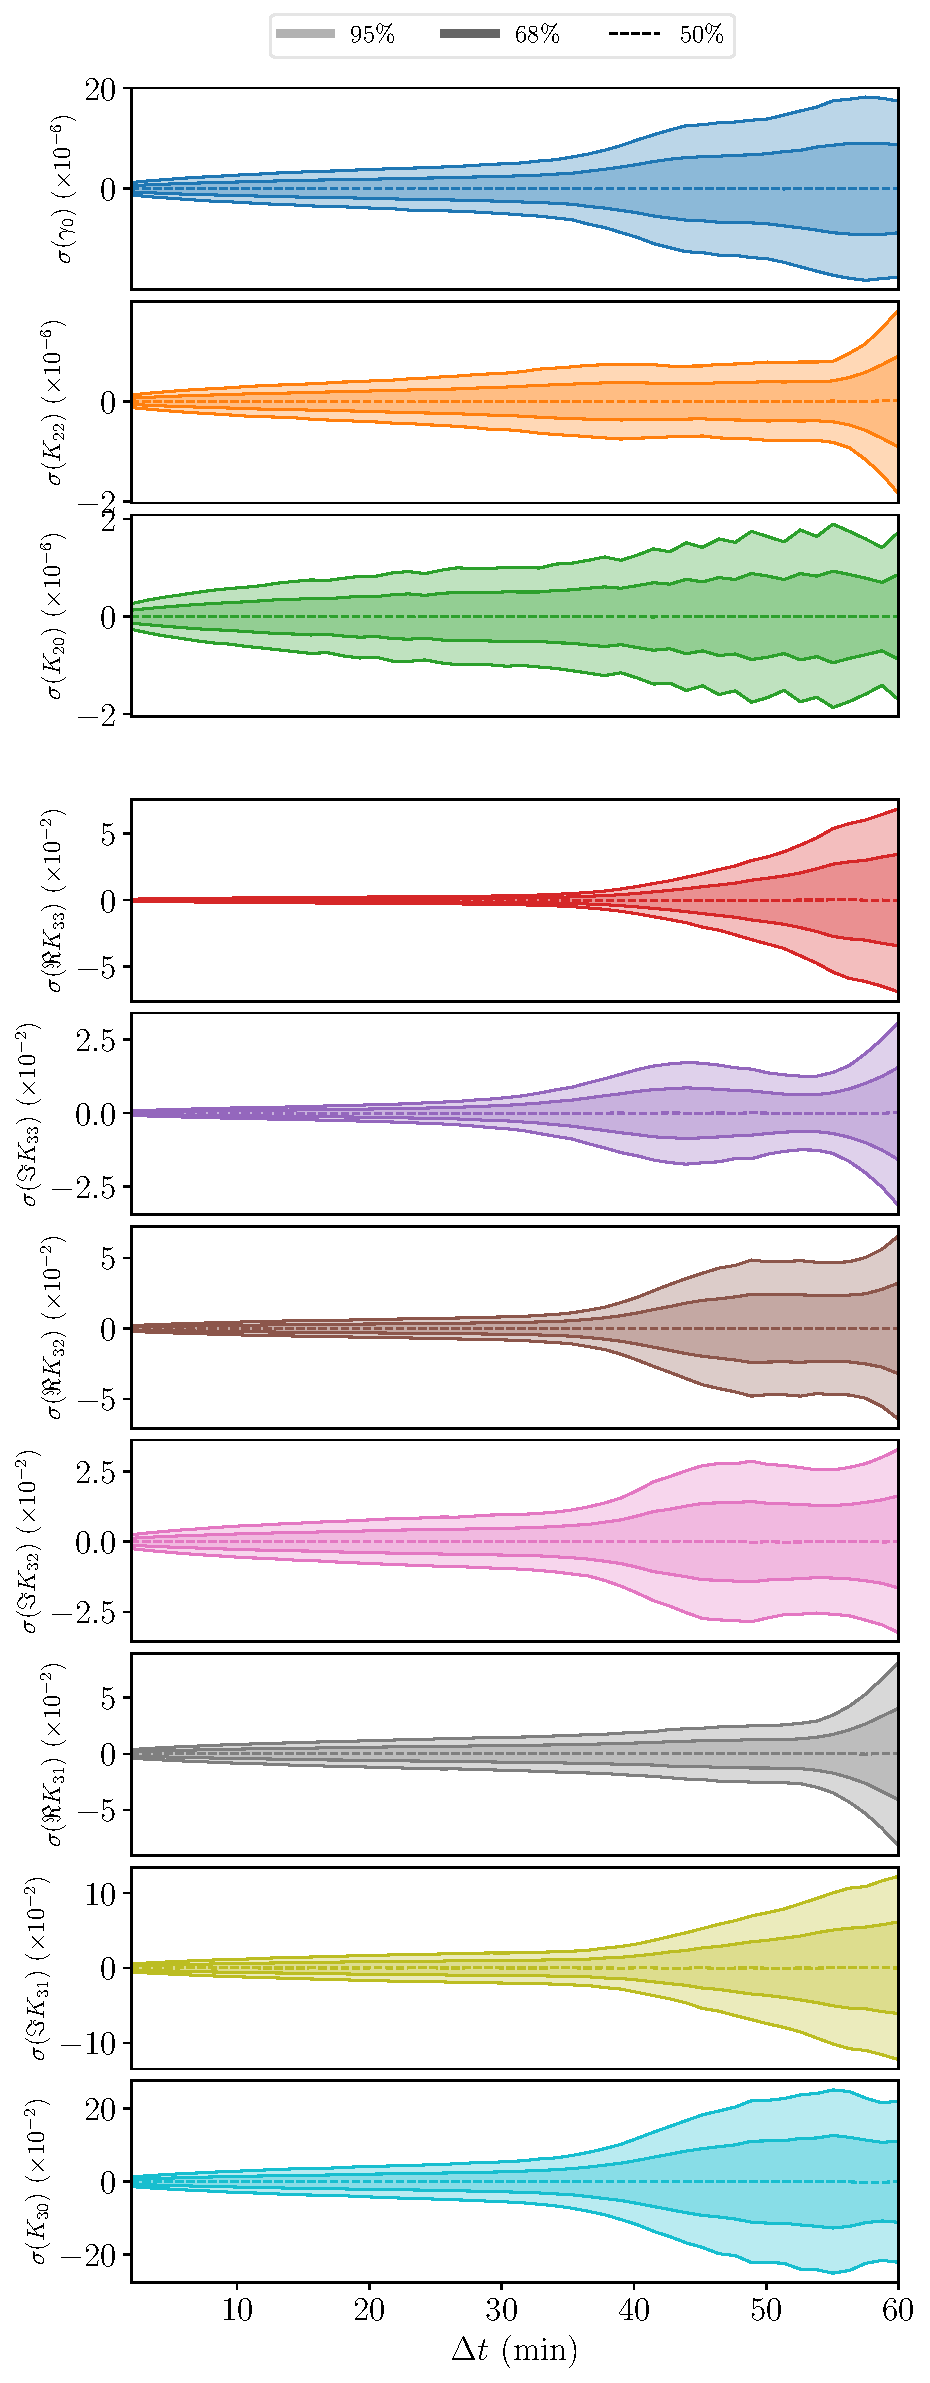
\includegraphics[height=0.89\textheight]{figs/scan-cadence.pdf}
  \caption{1 and 2$\sigma$ confidence intervals for the first-order parameter PPDs (\textit{top}) and second-order parameters (\textit{bottom}) as a function of observational cadence $\Delta t$ The reference cadence is 2 minutes. The red vertical lines indicate when $\sigma = 0.01$.}
  \label{fig:scan-cadence}
\end{figure}

Figure \ref{fig:scan-cadence} displays little dependence of uncertainty on cadence $\Delta t$ for $\Delta t \lesssim 40$ min. We also see flaring of uncertainty for very large cadence, largely driven by the paucity of data points. However, uncertainty dramatically increases for many parameters at about $\Delta t = 30-40$ min, a time scale which is likely characteristic of the asteroid system. We name this rough cadence limit $T_\text{cad}$.

We expect $T_\text{cad}$ to be a function of two dynamical time scales of the system: the rotational period of the asteroid $P_\omega$ and the time spent near perigee $T_p$. The latter can be estimated by
\begin{equation}
  T_p \sim \frac{r_p}{v_\infty}\brackets{2\frac{\mu_\mathcal{B}}{r_pv_\infty^2}+1}^{-\frac{1}{2}}
  \label{eqn:tp}
\end{equation}
which is the ratio of the perigee radius to velocity at perigee. The exact choice of the formula of $T_p$ not obvious, and alternatives to equation \ref{eqn:tp} are possible. For the simulated asteroid, $P_\omega = 9$ hr and $T_p = 42$ min by this definition.

We further study the effect of $P_\omega$ and $T_p$ on $T_\text{cad}$ in appendix \ref{app:cadence-tests}, and find that both affect $T_\text{cad}$ by roughly the same amount.

Figure \ref{fig:scan-cadence} shows that as long as $\Delta t < T_\text{cad}$ is achieved, the influence of cadence on $\sigma$ is minimal (except for $K_{30}$ where the $\sigma<0.01$ limit is slightly exceeded). However, shorter cadence almost always leads to lower uncertainties.



\subsection{Perigee gap}
\label{sec:scan-gap}
In certain circumstances, spin data might not be able to be captured for a close encounter at perigee. The asteroid might dip below the horizon, or it might pass too close to the sun to be observed. Generally, angular velocity data can be collected when the asteroid is distant from the central body, where torque is low. There, the angular velocity evolution is dominated by torque-free precession dictated by the moment of inertia components. That zero-torque data can still be used to fix $K_{20}$ and $K_{22}$ as in \cite{MOSKOVITZ2020113519}. However, $K_{3m}$ are not extractable from precession data alone. We are therefore curious as to how our posterior uncertainties change due to lack of data during the encounter perigee.

To test this, we mask the perigee of the counter by removing a duration $T$ of data centred on the perigee, where $T$ ranges from 0 to 3 hours. To prevent lack of precision on $K_{\ell m}$ induced by lower amounts of data for high $T$, we always cut 3 hr$-T$ from the data set, half from the beginning and half from the end, so that each data set produced for all $T$ has the same length of data before and after the perigee. We then fit the same asteroid model to the cut data for all $T$ and plot posterior uncertainties $\sigma$ in figure \ref{fig:observation-gap}.

\begin{figure}
  \centering
  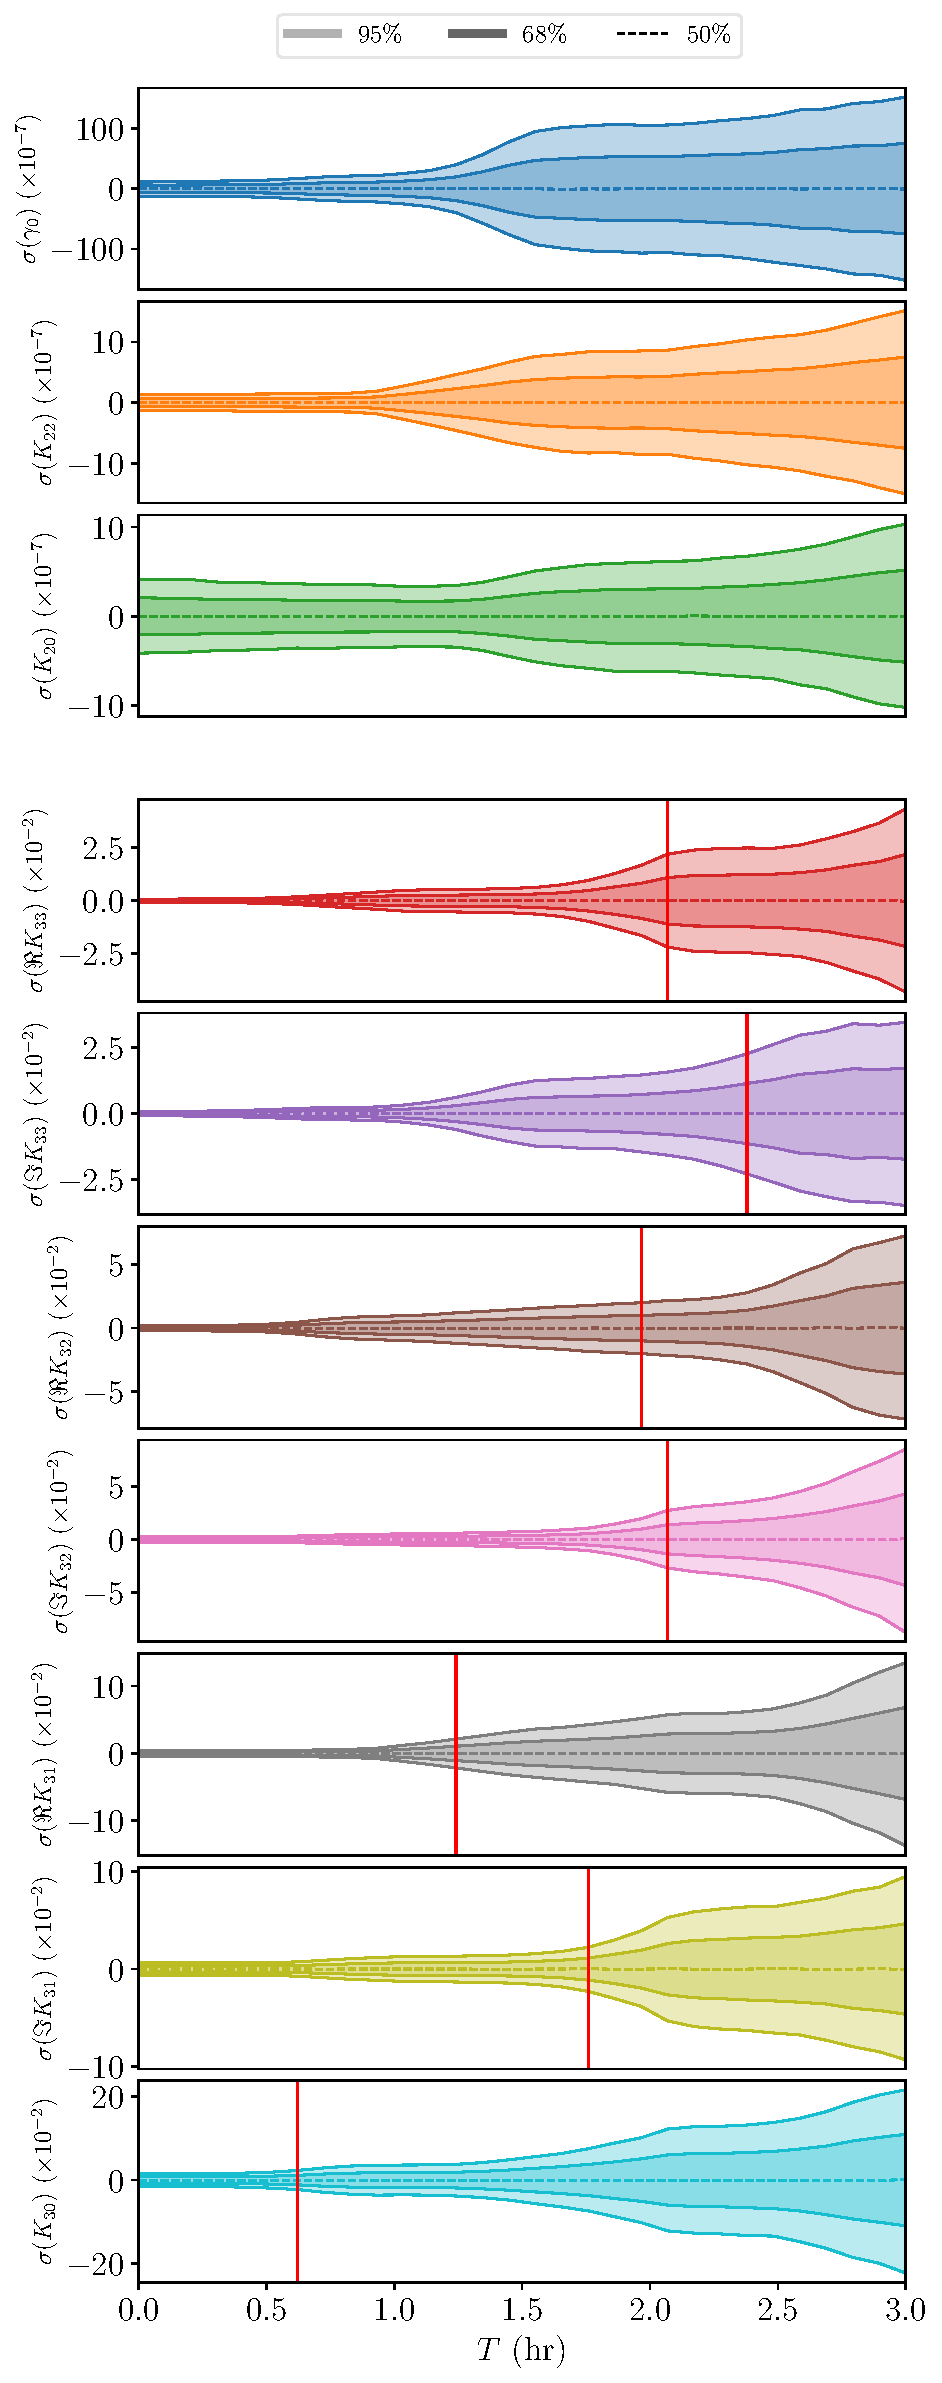
\includegraphics[height=0.89\textheight]{figs/observation-gap.pdf}
  \caption{1 and 2$\sigma$ confidence intervals for the first-order parameter PPDs (\textit{top}) and second-order parameters (\textit{bottom}) as a function of a data gap of width $T$ at perigee. The red vertical lines indicate when $\sigma = 0.01$.}
  \label{fig:observation-gap}
\end{figure}

Since torque is greatest at perigee, we expect that region of the data to contain the most information about $K_{\ell m}$, and therefore uncertainty should increase monotonically with $T$, which is seen in figure \ref{fig:observation-gap}. We also see that the first-order parameters are not as sensitive to $T$ as the second-order parameters, because $K_{2m}$ are additionally constrained by torque-free precession after perigee.

Most parameters show dramatically increased uncertainty in the $T \sim 1-2$ hr range. On the other hand, none of the uncertainties increase noticeably for $T < 30$ min. Thirty minutes of dropped data is equivalent to fifteen dropped points for the simulated cadence of $\Delta t = 2$ minutes, showing that many data points can dropped from the data set at perigee before the uncertainty starts to increase.

Qualitatively, \ref{fig:observation-gap} shows similar dependence of $\sigma$ on $T$ as \ref{fig:scan-cadence} showed for $\sigma$ on cadence $\Delta t$. They also both have cut-offs where uncertainty markedly increases, and both the $T$ and $\Delta t$ cut-offs have qualitatively similar shapes although they occur at different values of $\Delta t$ and $T$. This suggests that the factors that govern uncertainty due to cadence (appendix \ref{app:cadence-tests}) also may govern sensitivity to lack of data at perigee in a similar way.


\subsection{Initial spin pole}
\label{sec:scan-spin}

The tidal torque experienced by the asteroid is affected by the initial direction of asteroid spin $\bm \Omega_0$ both because spin sets the initial asteroid orientation up to $\gamma_0$ and because of the spin-dependence of the rotational equations of motion (equation \ref{eqn:omega-eom}).

In figure \ref{fig:scan-spin}, we display 1$\sigma$ uncertainties for all parameters as a function of the direction of $\bm \Omega_0$, mapped onto the unit sphere in the inertial frame. Our samples for $\bm \Omega_0$ were laid out on a Fibonacci sphere to ensure they were roughly evenly spaced (marked in figure \ref{fig:scan-spin-avg}). To highlight common features across the parameters, we also display the average 1$\sigma$ sensitivity in figure \ref{fig:scan-spin-avg}. The average is weighted such that the uncertainty map for each parameter contributes an equal amount
(the weight of each map is set to one-tenth of the map's mean). This average map is presented in two different projections to allow data at $\unit Z$ to be read.

\begin{figure*}
  \centering
  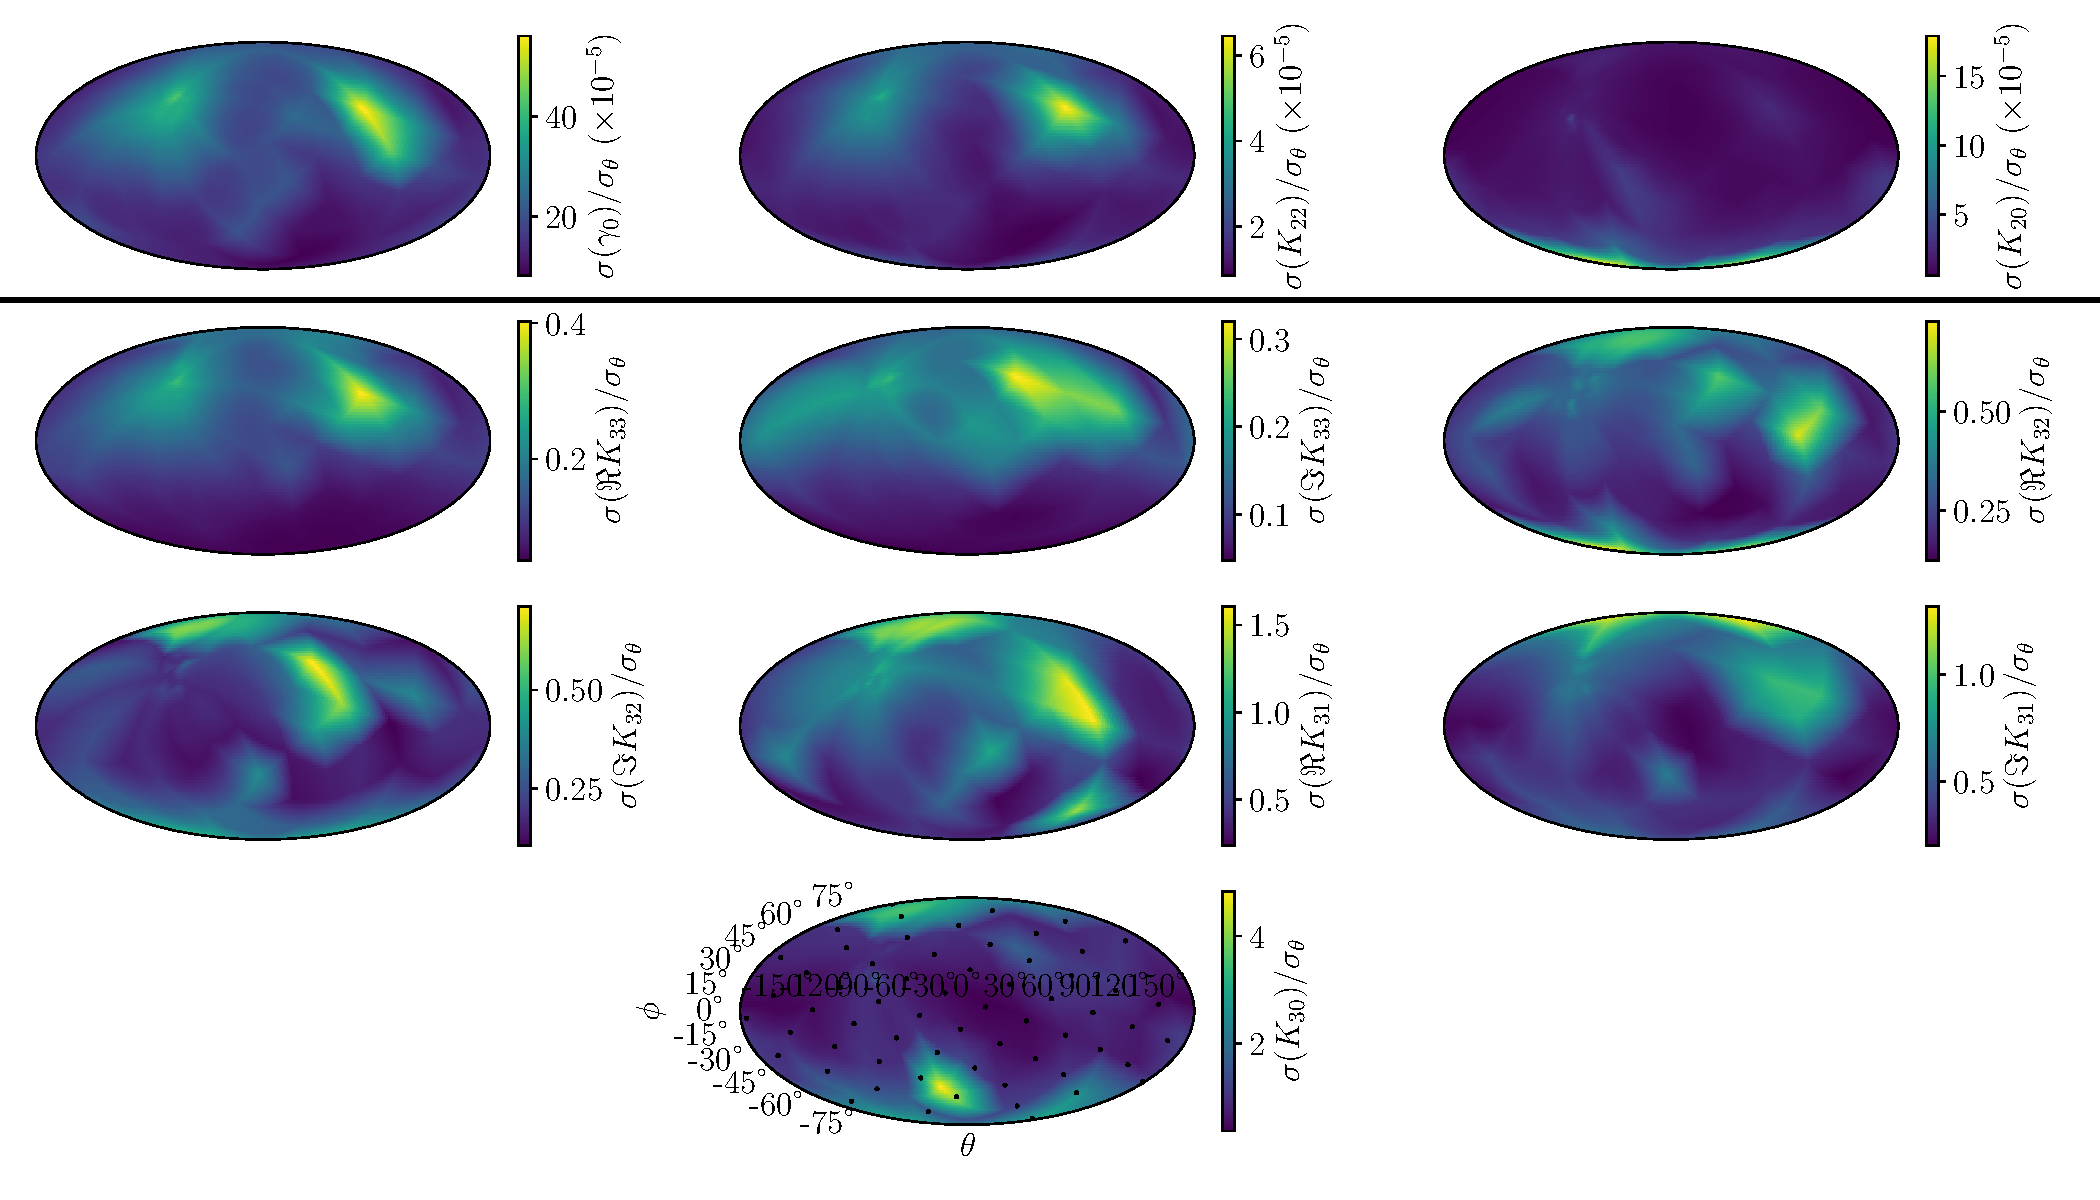
\includegraphics[width=\textwidth]{figs/spin-pole.pdf}
  \caption{$1\sigma$ uncertainties for the first-order parameters (\textit{top}) and second-order (\textit{bottom}) as a function of the initial direction of spin in the inertial frame. All maps are made in the Mollweide projection. The orange star indicates the reference spin pole. The red contours enclose regions where $\sigma \geq 0.01$.}
  \label{fig:scan-spin}
\end{figure*}

\begin{figure*}
  \centering
  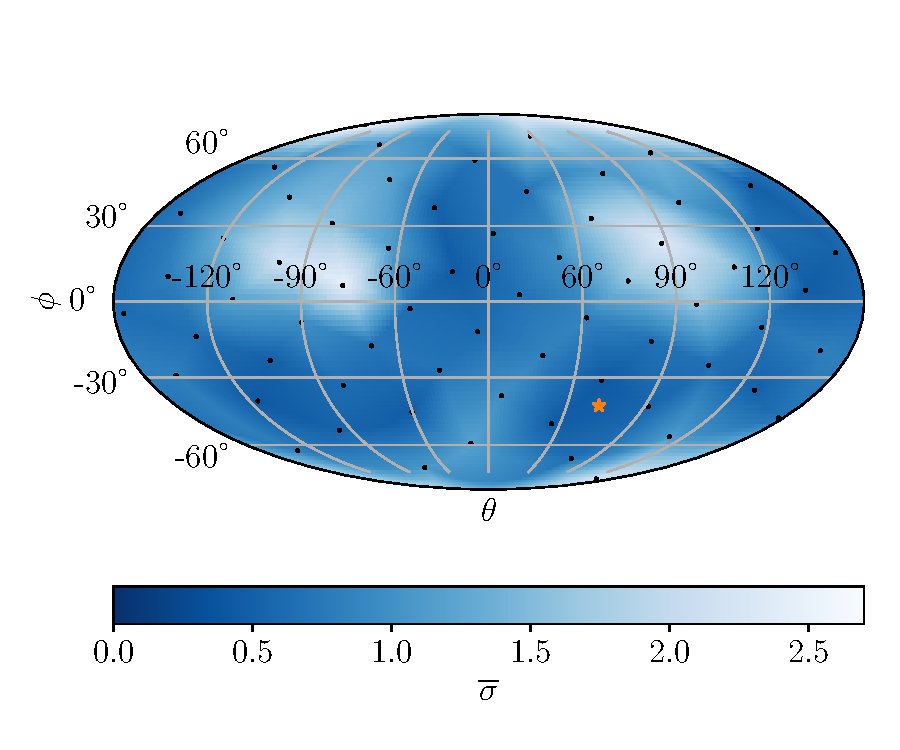
\includegraphics[width=0.45\textwidth]{figs/spin-pole-avg-mollweide.pdf}
  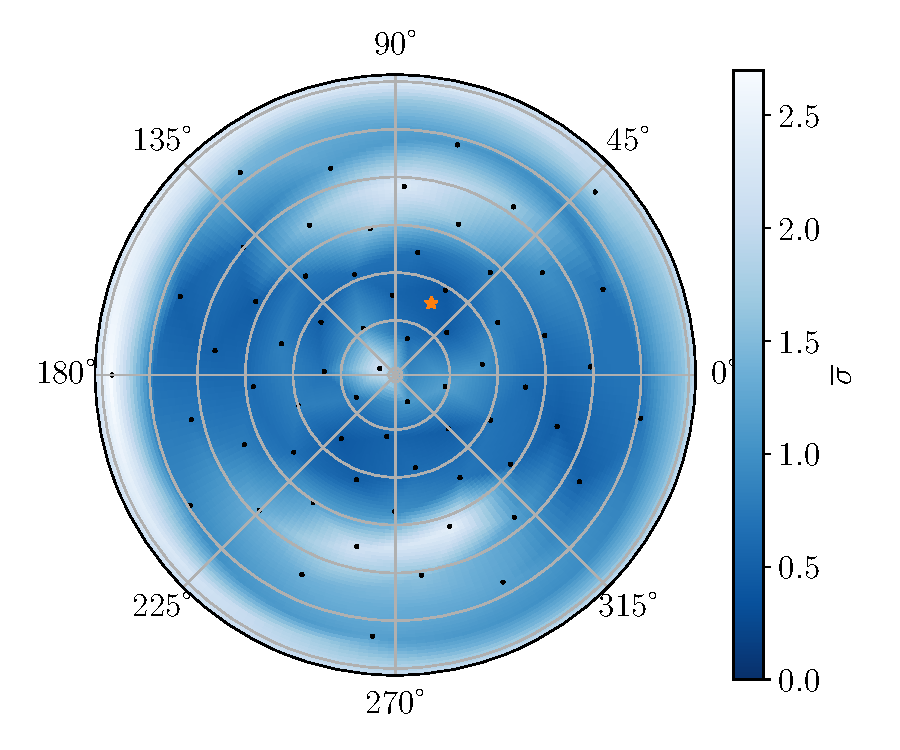
\includegraphics[width=0.45\textwidth]{figs/spin-pole-avg-polar.pdf}
  \caption{The weighted average of the uncertainties shown in figure \ref{fig:scan-spin}, in Mollweide (\textit{left}) and polar (\textit{right}) projections in the inertial frame. See text for a description of how the average was computed. Black dots indicate the Fibonacci-sphere-distributed locations of sample spin poles, and the orange star indicates the reference spin pole. The polar projection is centred at the south pole, or $-\unit Z$.}
  \label{fig:scan-spin-avg}
\end{figure*}

Certain alignments of the body-fixed frame to the inertial frame lead to special conditions on torque, as discussed in section \ref{sec:tidal-torque}. For example, $\bm z \parallel \unit Z$ and $\bm z \parallel \unit Y$ at perigee lead to $\bm \tau \parallel \unit z$ to first-order, and $\bm \tau \parallel \unit X$ at perigee leads to $\bm \tau = 0$ to first-order. We relate this to the initial direction of $\bm \Omega_0$, via the approximation that $\bm \tau$ is small until perigee. Then, since $\bm \omega_0 \parallel \unit z$ in the body-fixed frame as an initial condition (section \ref{sec:sim}), we have that $\bm \Omega_0 \parallel \unit Y$ and $\bm \Omega_0 \parallel \unit Z$ both lead to $\bm \tau \parallel \unit z$, and $\bm \Omega_0 \parallel \unit X$ leads to $\bm \tau = 0$.

Figure \ref{fig:scan-spin-avg} shows area of increased uncertainty for $\bm \Omega_0 \parallel \unit Z$ and $\bm \Omega_0 \parallel \unit Y$, but not the $\unit X$ case. This indicates that $\bm \tau \parallel \unit z$ causes increased uncertainty. Physically, $\bm \tau \parallel \unit z$ only changes an asteroid's rotational period and does not cause it to tumble, eliminating the ability to discern moment of inertia ratios from zero-torque precession after the encounter. Also, $\tau_z$ affected by fewer parameters than $\tau_x$ or $\tau_y$.  Both of these are reasons why $\bm \tau \parallel \unit z$ might inhibit precise fits to spin data. If $\bm \tau = 0$ to first-order, then second-order $\bm \tau$ and non-perigee $\bm \tau$ will dominate, which may increase precision to these usually non-dominant parameters and therefore not have the same increasing effect on $\sigma$.

It is important to note, however, that uncertainty does not vary by much more than a factor of two outside the imprecise regions of $\bm \Omega_0 \parallel \unit Z$ and $\bm \Omega_0 \parallel \unit Y$, though these regions are wide for some parameters. Within the imprecise regions, uncertainty can grow up to four times or more the uncertainty at other $\bm \Omega_0$ values, and can exceed the $\sigma ~0.01$ benchmark. The trends for are roughly consistent across parameters (figure \ref{fig:scan-spin}), leading to clearly visible imprecise regions in the average $\sigma$ (figure \ref{fig:scan-spin-avg}).




\subsection{Rotational period}
\label{sec:scan-period}

We also study the effect of the initial rotational period of the asteroid $P_\omega$ on posterior uncertainty $\sigma$. The dynamical time scales $r_p/v_\infty$ and $\mu_\mathcal{B} / (r_p v_\infty)$ have already been mentioned in the context of the cadence cut-off (section \ref{sec:scan-cadence}), and the ratio between them and $P_\omega$ in principal may affect $\sigma$. In figure \ref{fig:scan-period}, we show $\sigma$ as a function of $P_\omega$ for a range of periods typical of NEOs.

\begin{figure}
  \centering
  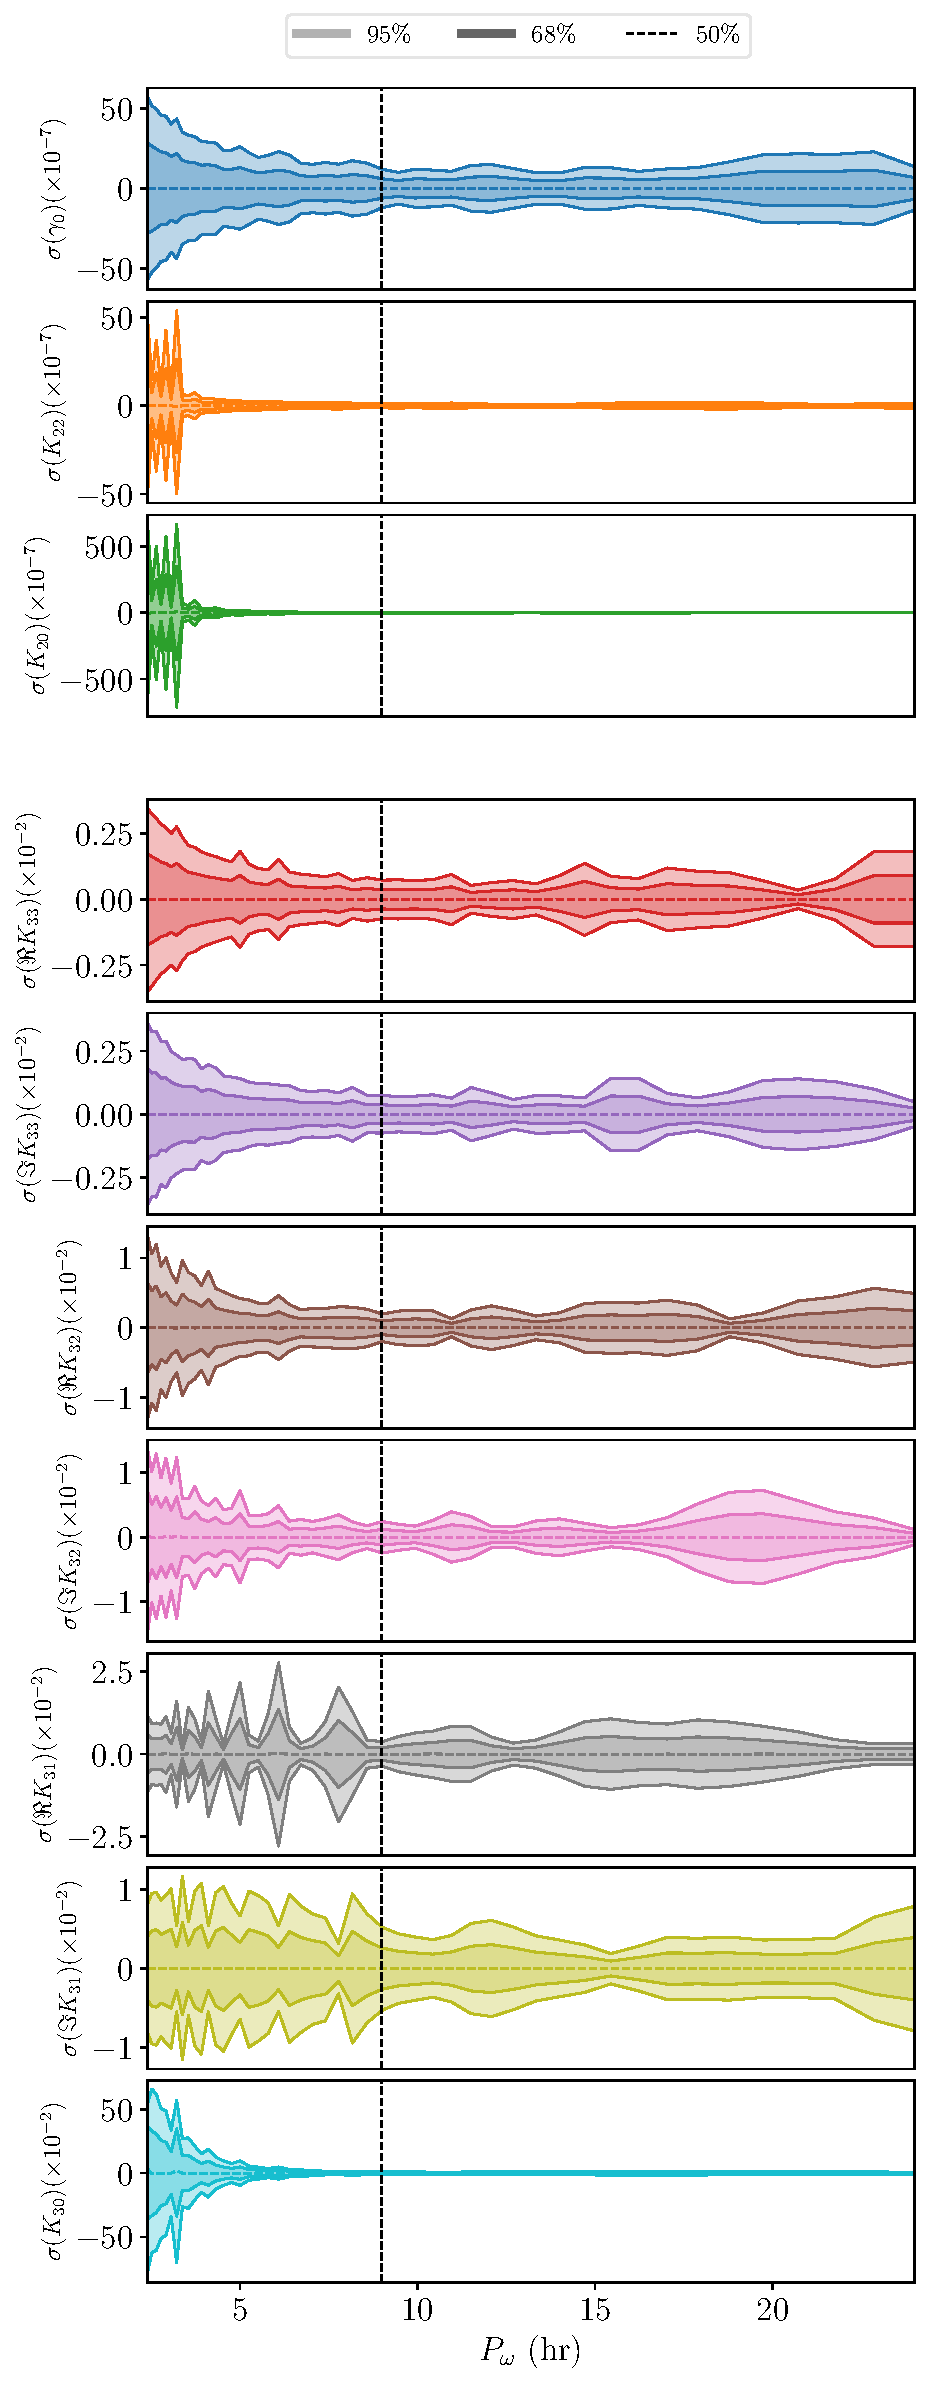
\includegraphics[height=0.89\textheight]{figs/scan-period.pdf}
  \caption{1 and 2$\sigma$ confidence intervals for the first-order parameter PPDs (\textit{top}) and second-order parameters (\textit{bottom}) as a function of initial rotational period $P_\omega$. The reference value of 9 hr is shown as a vertical dotted line. The red vertical lines indicate when $\sigma = 0.01$.}
  \label{fig:scan-period}
\end{figure}

Like figure \ref{fig:scan-vex}, depicting the dependence of $\sigma$ on $v_\infty$, figure \ref{fig:scan-period} shows small-scale variation in uncertainty due to the fact that varying the initial period changes the value of $\gamma$ at perigee, which affects uncertainty to a factor of about two. But a large-scale trend is also visible in many parameters. $K_{20}$ and $K_{22}$ show very large uncertainty for $P_\omega \lesssim 4$ hr because these fast-rotators tumble very little after perigee. This increases uncertainty on the $K_{2m}$ parameters, which are constrained by tumbling.

We expect that quickly rotating asteroids would not tumble because, for small $P_\omega$, the dynamical variables $\bm D$, $\bm \omega$, $\alpha$, and $\beta$ vary much smaller than $\gamma$. Approximating each variable as constant over one full rotation of $\gamma$, we can integrate the first-order contribution of $\bm \tau$ over $\gamma \in (0, 2\pi)$ and reveal that each rotation has zero average first-order torque. Since the first-order torque over each rotational period cancels out, there is no secular torque to force the asteroid to tumble. However, this effect does not apply to the second-order parameters, since the integral over the second-order term of $\bm \tau$ does not vanish, as seen in the figure.

Another feature of figure \ref{fig:scan-period} is that $K_{\ell 0}$ is more uncertain at low $P_\omega$ than the other parameters. This is most visible in the figure for $K_{30}$. The cause is likely that $K_{\ell 0}$ cannot contribute to $\tau_z$ as shown in equation \ref{eqn:tidal-torque}. We already discussed that asteroids with small $P_\omega$ do not tumble, and since $\tau_x$ and $\tau_y$ are what induces tumbling, the most observable component of torque is therefore $\tau_z$, which $K_{\ell 0}$ do not affect.

The most severe effect of period on $\sigma$ is in the low-period regime ($P_\omega \lesssim 5$ hr), but in this case, the most strongly affected parameters are $K_{2m}$, which are generally known better than $K_{3m}$. The effect on the imprecise parameters $K_{3m}$ is small, except for $K_{30}$. It therefore seems as though small-period asteroids are still candidates for observation, although high-period asteroids still have better uncertainty.


\subsection{Central body oblateness}
\label{sec:scan-oblateness}

In all the above studies, we assumed a spherical planet ($J_{\ell m} = 0$ for $\ell \geq 1$). By assumption that $\mu_\mathcal{B} \gg \mu_\mathcal{A}$ (so that the asteroid orbit's focus is the centre of mass of the central body), we have $J_{1m} = 0$. The effect of central body oblateness, then, is limited to the $J_{2m}$ terms, and therefore damped by a factor of $(a_\mathcal{B} / D)^2$. We expect these parameters to have little effect on the asteroid.

Here, we define oblateness as $\epsilon = (I_z - I_x)/(\mu_\mathcal{B} R_M^2)$, where $I_{x,y,z}$ are the central body moments of inertia along the principal axes, and $I_x = I_y$. $R_M$ is the true radius of the body (not $a_\mathcal{B}$ from equation \ref{eqn:jlm}). 

$J_{\ell m}$ is defined in equation \ref{eqn:jlm} with respect to the asteroid orbit, not the principal axes of the central body. However, for an equatorial orbit, the central body principal axes coincide with the asteroid orbit frame and we may express $\epsilon$ simply in terms of $J_{\ell m}$ as $\epsilon = -2J_{20}$ and $J_{22} = 0$. (Some sources such as Ref.~\cite{paterLissauer2015} take $\epsilon=J_{20}$ as their definition of $J_{20}$). For simplicity, we use this equatorial orbit case. If the orbit is non-equatorial, the other $J_{2m}$ terms will be non-zero. Since an oblate ellipsoid is mirror-symmetric around all three axes, table \ref{tab:klm-symmetries} indicates that $J_{3m}$ are all zero. The next order of precision after this oblateness approximation is therefore $J_{4m}$, damped by an additional $(a_\mathcal{B}/D)^2$ factor, and  non-ellipsoid corrections to the central body shape.

Given this conversion between $\epsilon$ and $J_{20}$, we analyze posterior uncertainty $\sigma$ of the first-order parameters as a function of $\epsilon$ across a reasonable range of central body oblatenesses based on those of Solar System planets \cite{paterLissauer2015}. These uncertainties are shown in the top pane of figure \ref{fig:scan-oblateness}, together with linear best-fitting curves for $\sigma(\epsilon)$.

\begin{figure}
  \centering
  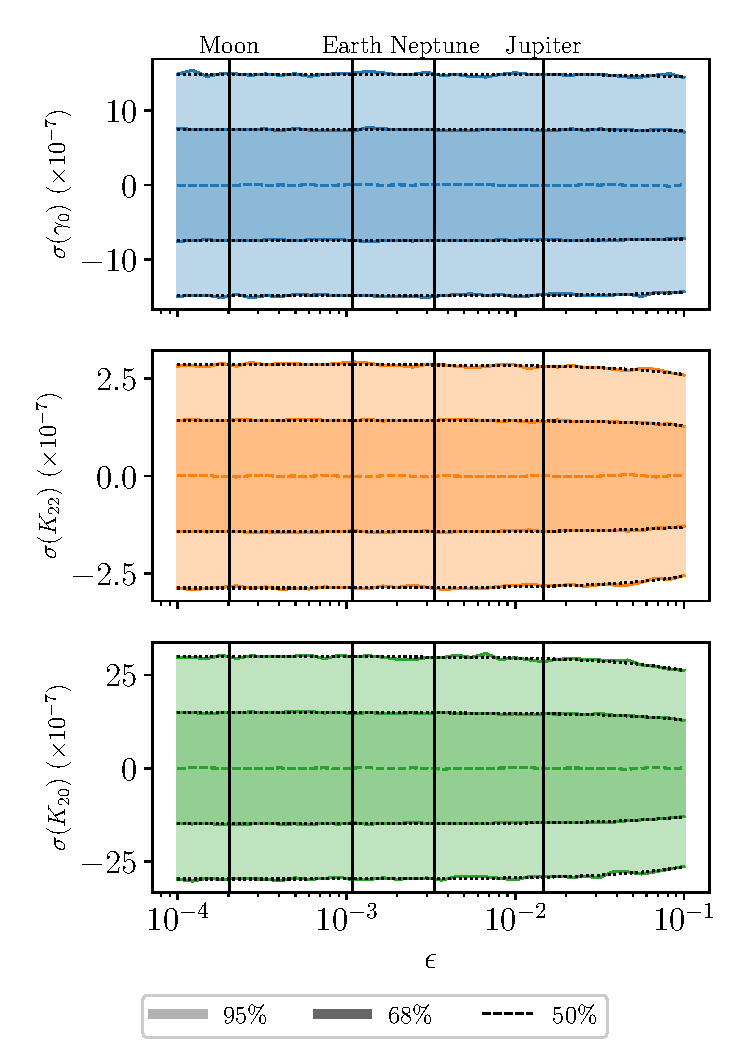
\includegraphics[width=0.88\columnwidth]{figs/oblateness.pdf}
  \vfill
  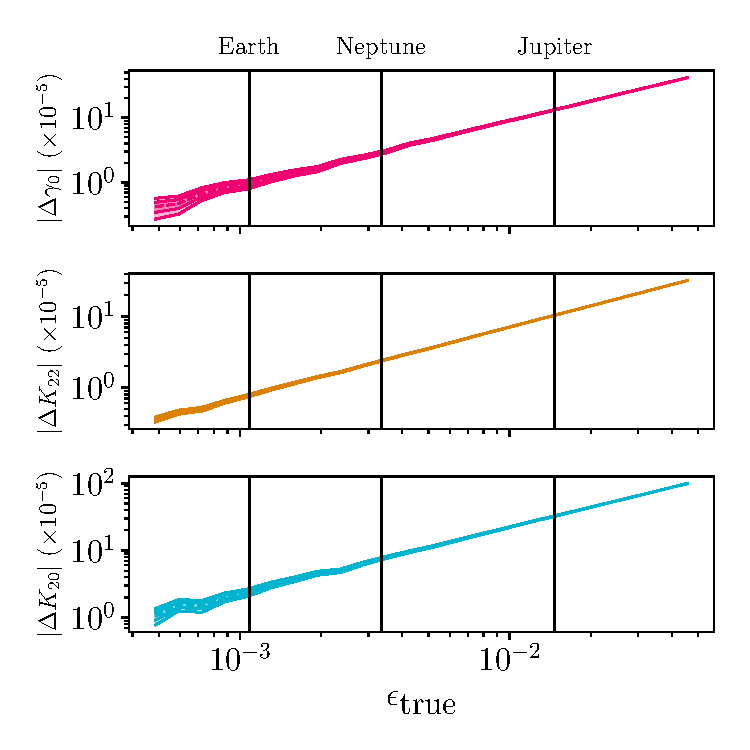
\includegraphics[width=0.88\columnwidth]{figs/oblateness-differ.pdf}
  \caption{\textit{Top}: 1 and 2$\sigma$ confidence intervals for the first-order parameter PPDs as a function of oblateness $\epsilon$ . Linear best-fitting lines to $\sigma$ (black, dotted) are plotted. \textit{Bottom}: The difference between PPD means extracted from a zero-oblateness model and the true parameters given data with true oblateness $\epsilon_\text{true} \neq 0$. Also shown in both figures are the oblatenesses of reference Solar System bodies.}
  \label{fig:scan-oblateness}
\end{figure}

The figure demonstrates a small dependence of $\sigma$ on oblateness $\epsilon$, but the effect is far from important compared to the other factors studied above. Most Solar System bodies do not reach the oblateness necessary to significantly increase precision on the first-order parameters. The best-fitting lines match the uncertainties well, and they have slope of $(\Delta \sigma / \sigma_{\epsilon=0}) / \Delta \epsilon = -0.26$ for $\gamma_0$, $-0.94$ for $K_{22}$, and $-1.2$ for $K_{20}$. The second-order parameters $K_{3m}$ likely depend on oblateness similarly, but fitting these parameters is computationally more expensive and we do not study them here.

Note that if an encounter is executed around one of the non-Earth objects noted in figure \ref{fig:scan-oblateness}, $a_\mathcal{B}$ and $\mu_\mathcal{B}$ will change in addition to $\epsilon$. These two parameters also affect the precision of the fit parameters (appendix \ref{app:jupiter-earth}), so the figure does not show that encounters with other bodies have the same precision as encounters with Earth; only that the difference in oblateness between the two bodies is of little concern.

Given the small effect of $\epsilon$ on $K_{\ell m}$, it might be tempting to neglect the planetary oblateness when fitting $K_{\ell m}$ to data. However, the bottom pane of figure \ref{fig:scan-oblateness} demonstrates that doing so is invalid. This figure displays $K_{\ell m}$ as extracted by a fit assuming $\epsilon = 0$, but run on data generated with non-zero $\epsilon$. The difference between the PPD means and true parameters are shown. Posterior uncertainties are also shown as bands. The figure shows that even for low (Moon-scale) oblateness, the fit results are inconsistent with the true $K_{\ell m}$ values, since $\Delta K_{\ell m} = 0$ is not contained in the 2$\sigma$ band. This effect is much worse for large oblateness, growing to a difference on the order of $10^{-2}$ between the true and fit parameters for large oblateness. Therefore, accurately modelling central-body oblateness to high precision is essential for accurate estimation of fit parameters. For non-equatorial orbits, with $J_{22} \neq 0$, we also expect $J_{22}$ to affect the accuracy of the fit results to a similar degree, with the additional requirement of using the correct asteroid orbital plane.

Note that $J_{20}$, the parameter studied in this section, has a slightly more general definition than oblateness. If the planet has a moon, the integral defining $J_{20}$ (equation \ref{eqn:jlm}) can be extended to include this extra mass. Since $J_{20}$ is a second moment, this effect is magnified for large distances of the mass from the central body centre of mass (though the effect is not quite quadratic because $a_\mathcal{B}$ also increases for large distances, and $J_{20}$ is divided by $a_\mathcal{B}^2$). This process is only valid when the asteroid never passes inside the moon's orbit.

As an order-of-magnitude estimate for this effect, two spherical objects with masses and radii of Earth and the Moon, separated by one Lunar distance, and both lying in the orbital plane has a combined $J_{20} = 0.25$. Extrapolating posterior uncertainty by the slopes of the best fit lines given earlier, this represents a decrease in $\sigma(K_{2m})$ by a factor of about one quarter.

This analysis suggests that large moons such as ours can improve fit quality, but further study of this effect is beyond the scope of this paper. Without a moon to inflate the oblateness of the central body, planetary oblateness does not significantly improve posterior uncertainty. However, correct representation of oblateness is essential to accurately estimate $K_{\ell m}$.





\section{The cadence cut-off}
\label{app:cadence-tests}

In section \ref{sec:scan-cadence}, we noted that posterior uncertainty as a function of observation cadence $\Delta t$ appears to increase suddenly near $\Delta t \sim T_\text{cad}=30-40$ min. We mentioned that this cadence cut-off is likely a function both of the rotational period of the asteroid and the time spent near perigee. We study this cut-off in closer detail in this appendix.

We measure the dependence of the cadence cut-off on rotational period by varying the period $P_\omega$ and reproducing figure \ref{fig:scan-cadence}; i.e., we run many simulations of the changed $P_\omega$ with different cadences and plot the posterior fit uncertainty $\sigma$ as a function of cadence $\Delta t$. Specifically, we use $P_\omega = 5$ hr and 20 hr, roughly double and half of the reference $P_\omega=9$ hr. The resulting curves of $\sigma(\Delta t)$ are shown in figure \ref{fig:cad-period}, with each normalized so that their maximum values is 1 so that changes to $\sigma$ induced by the change in $P_\omega$ that are not a function of $\Delta t$ (i.e., those studied in section \ref{sec:scan-period}), are removed; they are irrelevant here.

\begin{figure}
  \centering
  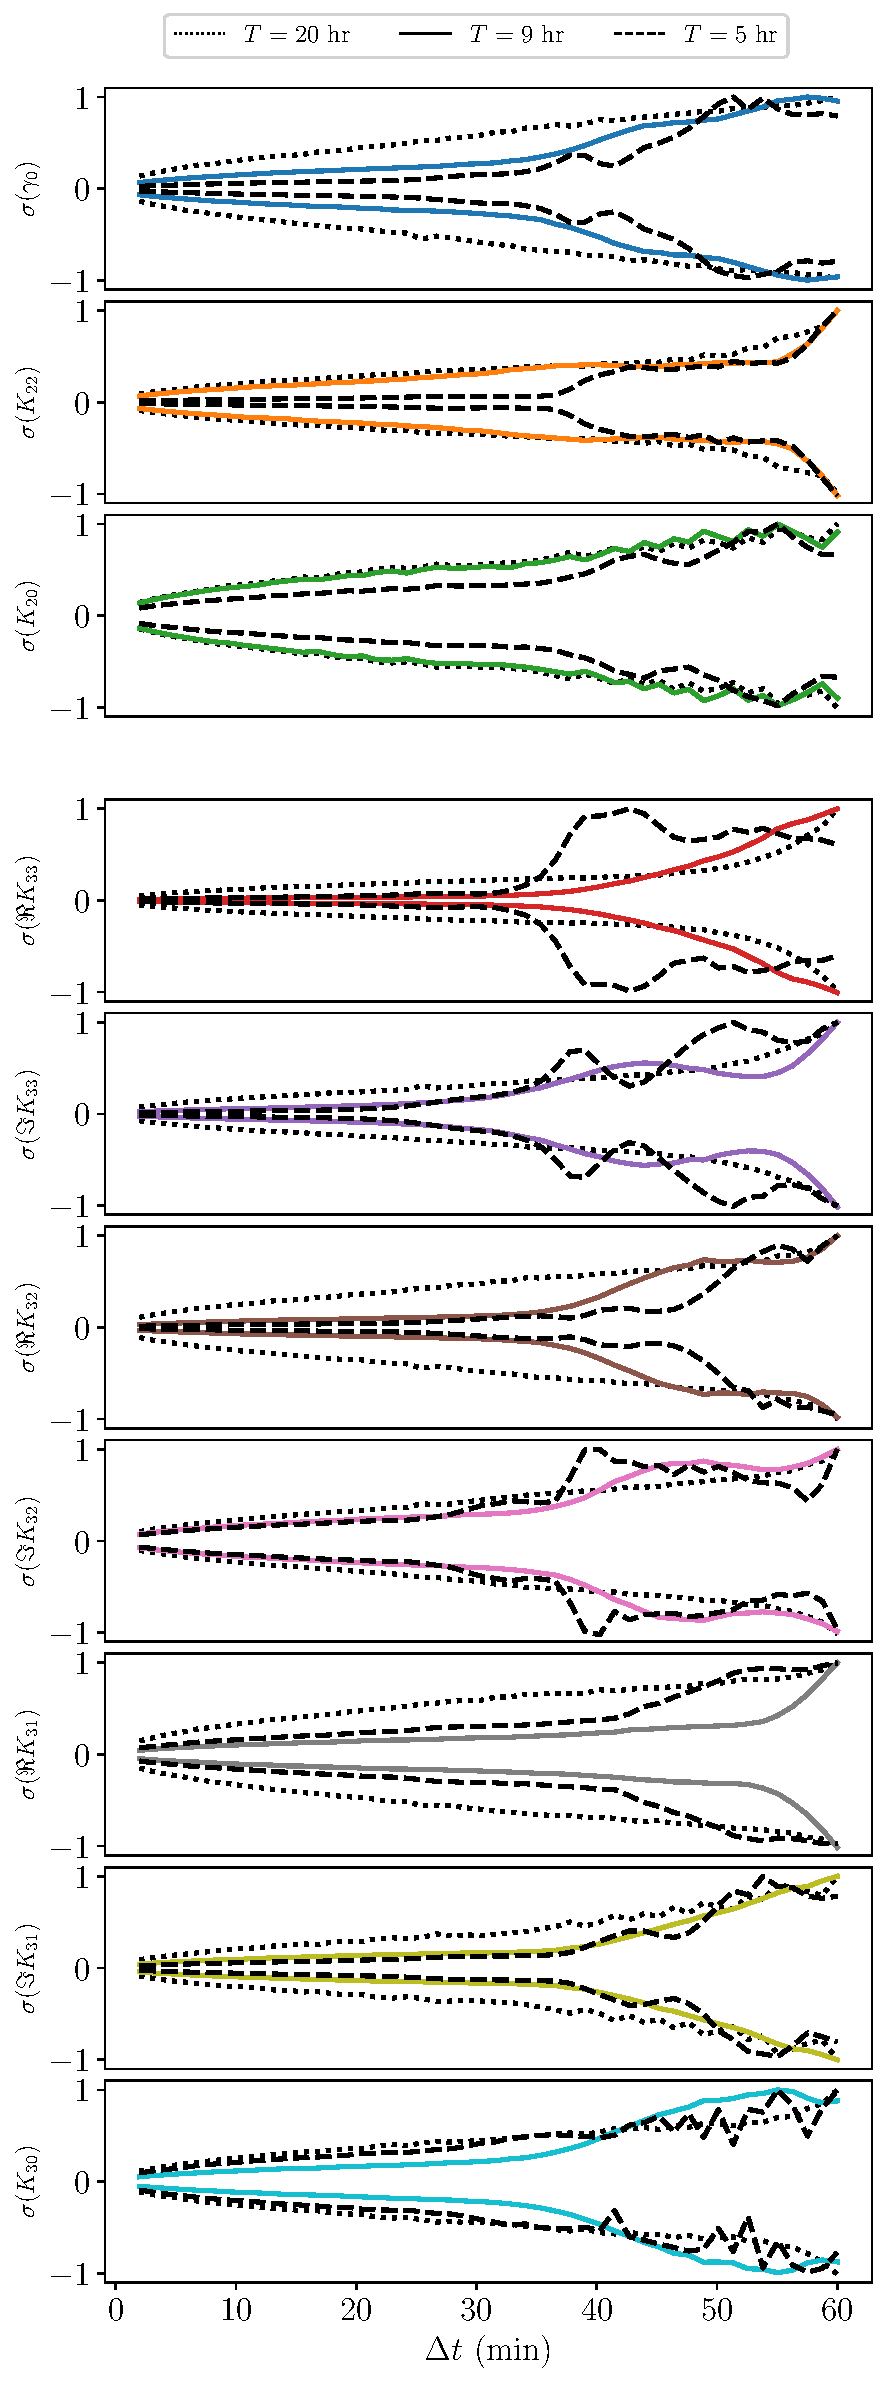
\includegraphics[height=0.89\textheight]{figs/cad-period.pdf}
  \caption{1$\sigma$ confidence intervals plotted as a function of cadence $\Delta t$ for periods of 9 hr (the reference asteroid, solid coloured lines), and 5 hours (dotted lines), and 20 hours (dashed lines). Confidence intervals have been normalized for the sake of comparison, so that the maximum for each curve is 1.}
  \label{fig:cad-period}
\end{figure}

We also wish to capture dependence on the time spent by the asteroid near perigee, but we do not wish to change the orbit shape or central body, because this may induce other effects that could also affect the cadence plot. Instead, we (un-physically) manipulate the speed at which the asteroid moves through the orbit. In one instance, the asteroid's path is artificially slowed by a factor of 2, which we denote as $t_\text{spin}/t_\text{orbit}=0.5$; in the other instance, $t_\text{spin}/t_\text{orbit}=2$, meaning that the orbit is sped up. This approach of changing the speed of the orbit is meant to approximate changes to $T_p$ defined in equation \ref{eqn:tp}. The posterior uncertainties for these two cases and the original case are shown as a function of $\Delta t$ in figure \ref{fig:cad-speed}. Again, $\sigma$ is normalized so that $\Delta t$-independent variations are removed. The $t_\text{spin}/t_\text{orbit}=2$ uncertainties begin to fill the prior distribution for large $\Delta t$ for some parameters, which can be seen by discontinuous variation in the dotted line of figure \ref{fig:cad-speed}.

\begin{figure}
  \centering
  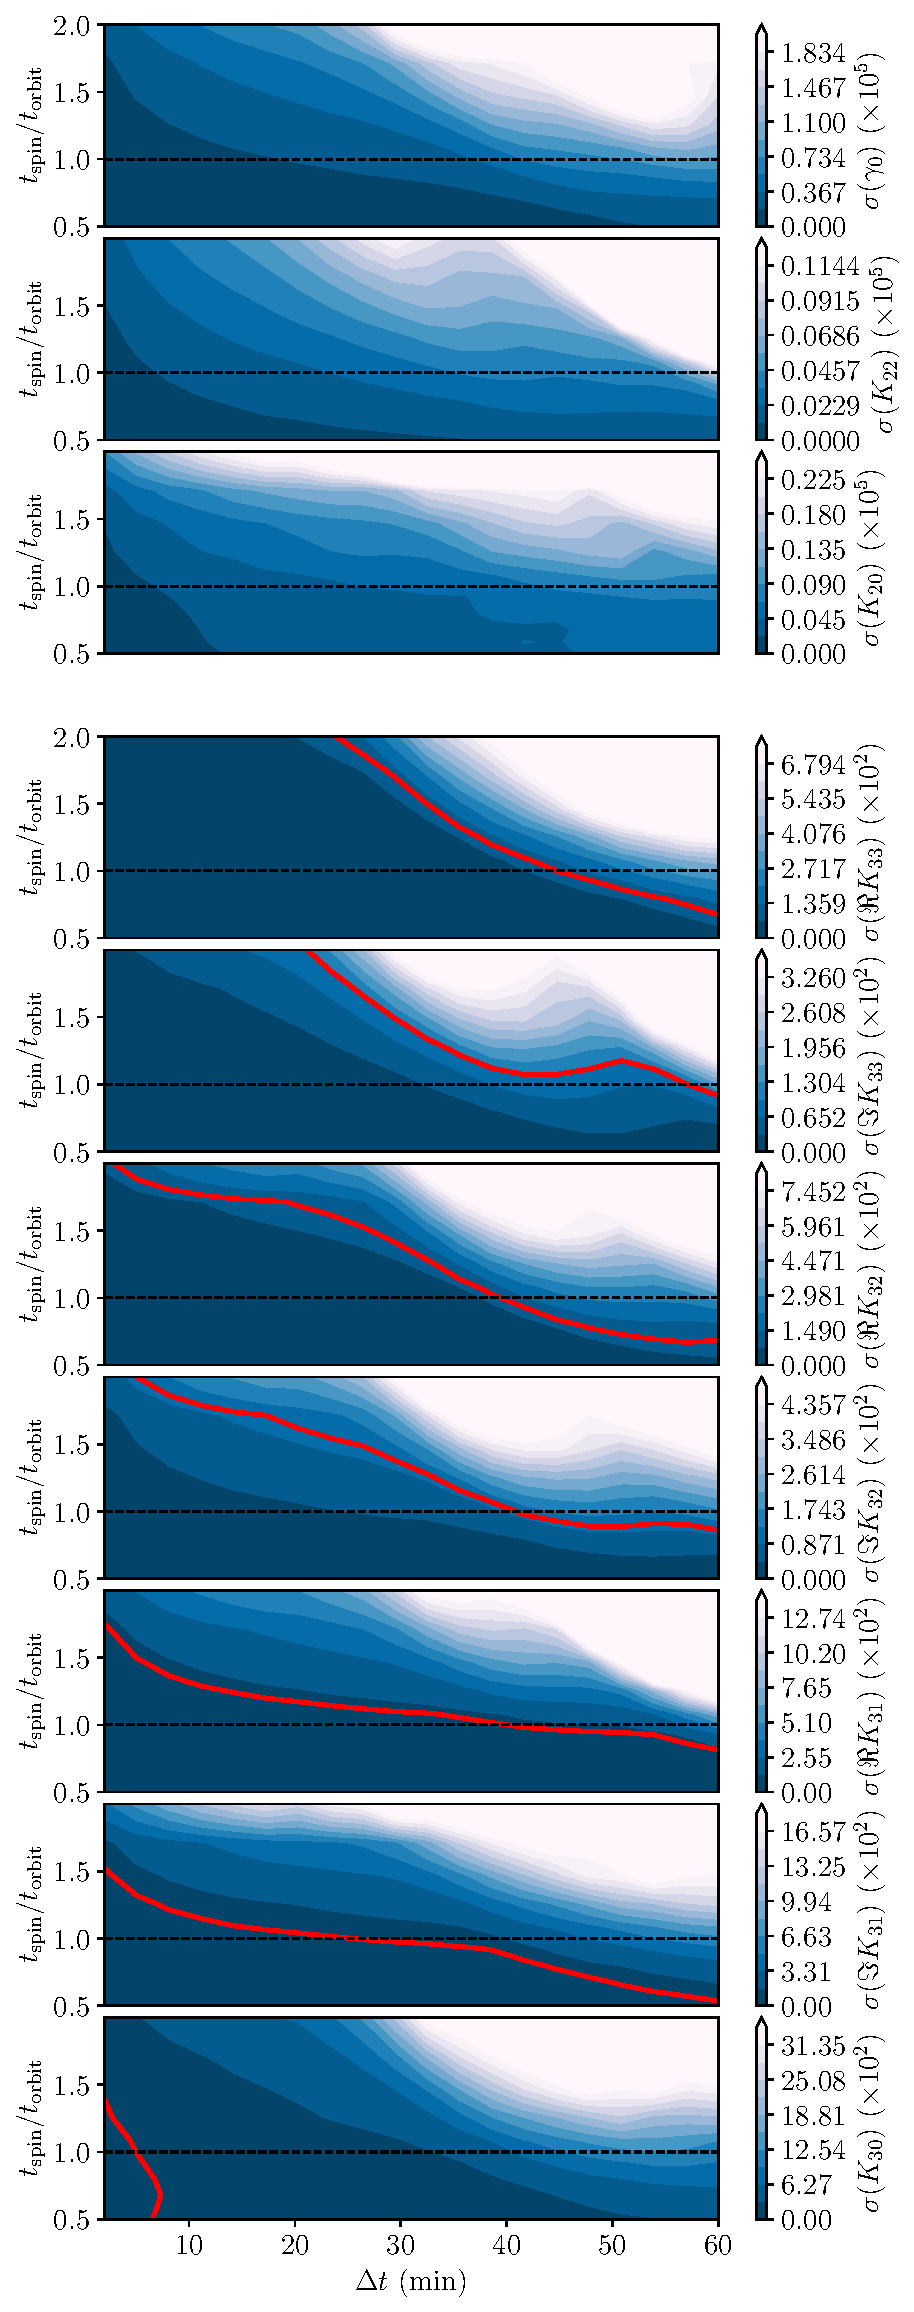
\includegraphics[height=0.89\textheight]{figs/cad-speed.pdf}
  \caption{1$\sigma$ confidence intervals plotted as a function of the orbit time scaling $t_\text{spin}/t_\text{orbit}$ for no scaling (the reference asteroid, solid coloured lines), time doubling (dotted lines), and halving (dashed lines). See text for the definition of $t_\text{spin}/t_\text{orbit}$. Confidence intervals have been normalized for the sake of comparison, so that the maximum for each curve is 1.}
  \label{fig:cad-speed}
\end{figure}

Many of the curves in figures \ref{fig:cad-period} and \ref{fig:cad-speed} show a cadence cut-off at $T_\text{cad} \sim 30-60$ min. Those that show no cut-off (i.e., they merely smoothly increase over $\Delta t$) may in fact exhibit a cut-off $T_\text{cad} > 60$ min, which is off the plot. By comparing $\sigma(\Delta t)$ for a specific parameter, we see that the dashed lines often (but not always) reach the cadence cut-off at lower $\Delta t$ than the solid line. For example, in figure \ref{fig:cad-period}, this effect is especially clear for $K_{22}$, $K_{33}$, $\Im K_{22}$, and $\Re K_{31}$, but the opposite appears for $\Re K_{32}$. The dashed curves are significant in both figures because they represent larger $\sigma$ cases ($P_\omega=5$ hours, or $t_\text{spin}/t_\text{orbit}=2$); section \ref{sec:scan-period} reveals that fast rotators lead to larger $\sigma$, and $t_\text{spin}/t_\text{orbit} > 1$ leads to larger $\sigma$ because of the presence of less perigee data. It therefore appears that small $P_\omega$ and small times spent at perigee move the cadence cut-off to smaller $T_\text{cad}$.

The dependence of the exact location of the cadence cut-off is likely more complicated than the above analysis indicates. However, large uncertainties induced by small $P_\omega$ or large $t_\text{spin}/t_\text{orbit}$ makes it difficult to produce data which are not affected by the finite size of the prior (as figure \ref{fig:scan-vex} is) to study these regimes. Computation time and random variation in $\sigma$ also limits us. We therefore do not attempt to explore the dependence between $T_\text{cad}$ and the encounter parameters further. If a future analysis does require a detailed understanding of how cadence affects uncertainty for a specific encounter, our simulation and fit process can be run given the parameters of the encounter in question in a similar manner to section \ref{sec:scan-cadence} to yield more information. 

  

\section{Computing asteroid shape from density moments}
\label{app:find-surface}

\begin{figure*}
  \centering
  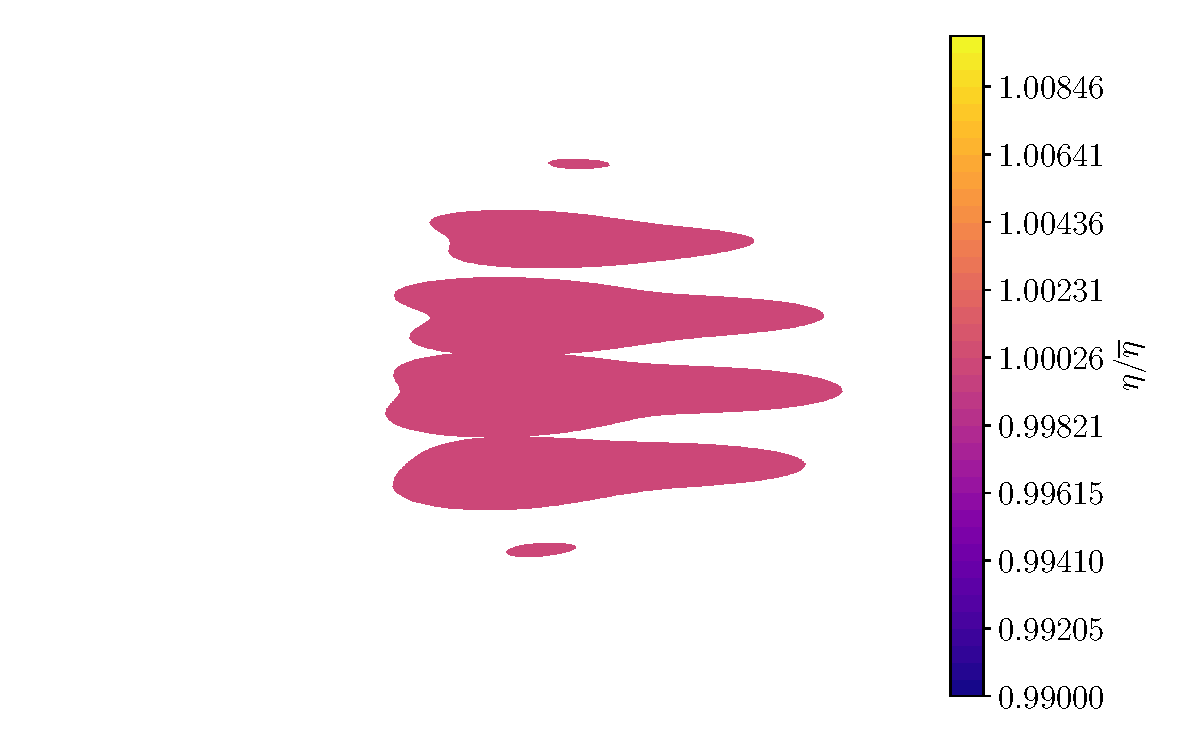
\includegraphics[width=0.45\textwidth]{figs/high-surface.pdf}\hfill
  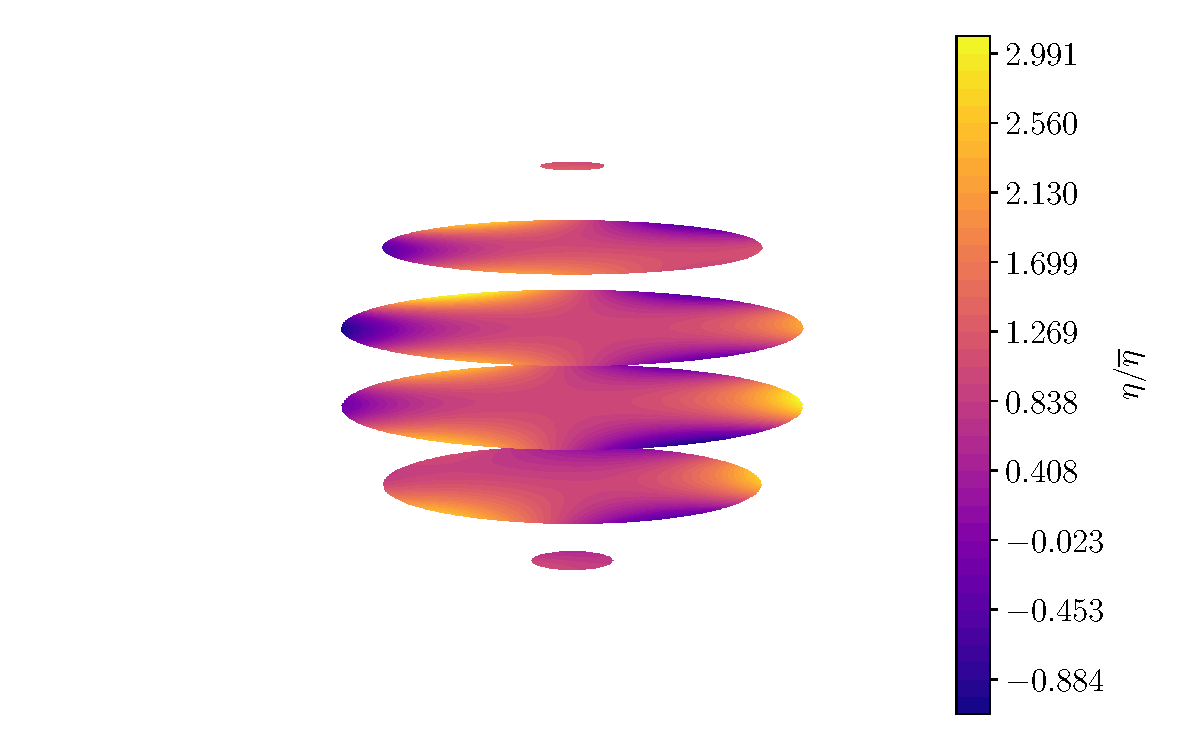
\includegraphics[width=0.45\textwidth]{figs/high-likelihood.pdf}
  \caption{\textit{Left}: the surface of a near-spherical asteroid with uniform density distribution extracted via the surface model. \textit{Right}: the density distribution extracted via the likelihood model for the same density moments but a spherical surface. The same length scale is used in both figures.}
  \label{fig:surface-density}
\end{figure*}

In section \ref{sec:general-density}, we mention that the shape of the asteroid can be computed from observations of the density moments and $a_\mathcal{A}$ if a uniform density distribution is assumed. We did not further describe the model in the main text because it is unlike the other three models in the nature of its assumptions, and in the fact that it is non-linear. However, it may be a useful technique so it is mentioned here; we call it the ``surface'' model. A similar model was also studied in Ref.~\cite{BAXANSKY2007756}.

Suppose our asteroid has constant density $\rho_0$ and known parameters $K_{\ell m}$ and $a_\mathcal{A}^2$, and that the asteroid is ``star shaped'' in that every ray originating from the centre of mass of the asteroid (the origin of the body-fixed frame) passes through the surface of the asteroid exactly once, at distance $r(\theta, \phi)$ written in spherical coordinates. By the divergence theorem, we write
\begin{equation}
  K_{\ell m} = \frac{\rho_0}{\mu_\mathcal{A} a_\mathcal{A}^\ell} \oint_{\partial \mathcal{A}} d^2 \bm r \cdot \bm v (\bm r)
\end{equation}
where $\bm v (\bm r) = \unit r R_{\ell m} (\bm r) r / (3+\ell) $ so that $\nabla \cdot \bm v(\bm r) = R_{\ell m}(\bm r)$. The integral is carried out over the surface of the asteroid. We know the area element satisfies $d^2 \bm r = (\partial \bm r / \partial \theta \times \partial \bm r / \partial \phi) d\theta d\phi$ in our coordinates, and when dotted with $\bm v \parallel \unit r$, this gives
\begin{equation}
  K_{\ell m} = \frac{\rho_0 }{\mu_\mathcal{A} a_\mathcal{A}^\ell (3 + \ell)} \int d\Omega r(\theta, \phi)^3 R_{\ell m}(r(\theta, \phi), \theta, \phi).
  \label{eqn:surface-klm}
\end{equation}
where the integral is carried out over the unit sphere. Note that the integrand of each $K_{\ell m}$ is proportional to $r(\theta, \phi)^{(3+\ell)}$ times constants and a spherical harmonic.

We write 
\begin{equation}
  r(\theta, \phi) = \sum_{\ell m} Y_{\ell m}^* C_{\ell m}
\end{equation}
without loss of generality. To keep $r(\theta, \phi) \in \mathds{R}$, we require $C_{\ell m}^* = (-1)^m C_{l,-m} (\ell-m)!/(\ell+m)$. With this definition, equation \ref{eqn:surface-klm} becomes a polynomial of degree $3+\ell$ in terms of $C_{\ell m}$ and integrals of products of spherical harmonics. These integrals can be pre-computed so that equation \ref{eqn:surface-klm} can then be numerically solved via standard polynomial solution methods to find $C_{\ell m}$. A similar equation to equation \ref{eqn:surface-klm} can be written for $a_\mathcal{A}$
\begin{equation}
  a_\mathcal{A}^2 = \frac{\rho_0}{5\mu_\mathcal{A}}\int d\Omega r(\theta, \phi)^5
  \label{eqn:surface-am}
\end{equation}
which can also be solved via polynomial methods.

Equations \ref{eqn:surface-klm} and \ref{eqn:surface-am} form a set of $n+1$ constraints, where $n$ is the number of density moments known. That is, $n=(\ell_\text{max}+1)^2+1$, where $\ell_\text{max}$ is the maximum degree of $K_{\ell m}$ known. By setting the same maximum degree on $C_{\ell m}$, we also have $n$ variables plus one for $\rho_0$. The system is therefore well-determined and will yield finitely many solutions. These solutions can be further refined by removing those that produce $r(\theta, \phi) < 0$ for any $\theta, \phi$, which is unphysical. We do not attempt to model uncertainty on the shape.

To test the model, this process was run for an asteroid with $K_{1m}=K_{2m'}=0$, but randomly chosen $K_{3m}$. The resulting surface is shown in figure \ref{fig:surface-density}. The figure shows a near-spherical asteroid, which is expected for $K_{\ell m} = 0$ for $\ell > 0$. However, the additional $K_{3m}$ components clearly induce non-sphericity in the asteroid which is captured by the surface model.

To give an alternate view of the non-sphericities found via this new surface model, figure \ref{fig:surface-density} also displays the density distribution extracted via the likelihood model assuming a spherical asteroid shape, but with the same density moments. (Uncertainty in the moments is not modelled in this figure, to better compare the two.) Where the likelihood model displays low density, the surface model clearly retracts into the asteroid. Where the likelihood model yields high density, the surface model extends. Thus, the connection made in section \ref{sec:spherical-density} between non-uniformities in the densities of the likelihood and harmonic models at the asteroid surface and inaccuracies in the surface is more firmly represented.

This surface model could, in principle, be used to improve estimates of the surface of an asteroid made by light curve analysis, since it connects rotational data to the asteroid surface which reflects the light we observe. Thus, uncertainties either in the density moments or the asteroid surface (or both), could be reduced. We only suggest this as a possibility, however, since light-curve analysis is beyond the scope of this paper.


\label{app:example}